% modded-nanoTabPFN --- Master's project presentation
% Beamer / metropolis. Build with: make  (latexmk + lualatex)
\documentclass[aspectratio=169,10pt]{beamer}

\usetheme{metropolis}
\metroset{progressbar=frametitle, numbering=fraction, block=fill}

\usepackage[T1]{fontenc}
\usepackage{booktabs}
\usepackage{amsmath,amssymb}
\usepackage{tikz}
\usetikzlibrary{positioning,arrows.meta,fit,backgrounds,calc,matrix}
\usepackage{pgfplots}
\pgfplotsset{compat=1.18}
\usepackage{xcolor}
\usepackage{xurl}
\usepackage{emoji}
\setemojifont{Noto Color Emoji}

% --- palette ---------------------------------------------------------------
\definecolor{accent}{HTML}{C1121F}      % speedrun red
\definecolor{ink}{HTML}{2B2D42}
\definecolor{muted}{HTML}{6C757D}
\definecolor{good}{HTML}{2A9D8F}
\setbeamercolor{frametitle}{bg=ink}
\setbeamercolor{background canvas}{bg=white}
\setbeamercolor{normal text}{fg=ink, bg=white}
\setbeamercolor{progress bar}{fg=accent}
\setbeamercolor{alerted text}{fg=accent}

\newcommand{\hl}[1]{{\color{accent}\textbf{#1}}}
\newcommand{\gd}[1]{{\color{good}\textbf{#1}}}
\newcommand{\mut}[1]{{\color{muted}#1}}

% compact citation marks (we keep refs informal on slides)
\newcommand{\cit}[1]{{\scriptsize\color{muted}[#1]}}

\title{modded-nanoTabPFN}
\subtitle{Tabular Foundation Model Pretraining Speedrun}
\author{Salih \underline{Bora} Öztürk}
\institute{University of Freiburg \\ \footnotesize Supervisor: Alexander Pfefferle \\ \footnotesize Examiner: Frank Hutter}
\date{11 June 2026}
\titlegraphic{%
  \begin{tikzpicture}[remember picture, overlay]
    \node[anchor=south east] at ([xshift=-8mm,yshift=6mm]current page.south east) {
\includegraphics[height=3cm]{img/logo_ufr.png}};
  \end{tikzpicture}%
}

\begin{document}

\maketitle

% ===========================================================================
\begin{frame}{Key message}
  \begin{itemize}
    \item We ran a speedrun for the tabular community.\\
      \hl{60--80$\times$} speedup
    \medskip
    \item What got us there:
    \begin{itemize}
      \item Brought proven tricks over from the other domains
      \item Reverified techniques from the tabular domain
    \end{itemize}
    \medskip
    \item There is so much left to discover, we never stop!
  \end{itemize}
\end{frame}

% ===========================================================================
\begin{frame}{Outline}
  \setbeamertemplate{section in toc}[sections numbered]
  \tableofcontents
\end{frame}

% ===========================================================================
\section{Speedrun Overview}

\begin{frame}{Pretraining is the faster-iteration bottleneck}
  \begin{itemize}
    \item TabPFN showed it: pretraining on \emph{synthetic} datasets gives strong tabular models. \cit{Hollmann '23/'25}
    \medskip
    \item But every new idea in
    \begin{itemize}
      \item architecture
      \item prior
      \item optimizer
    \end{itemize}
    needs a fresh pretraining run.
    \medskip
    \item And pretraining takes long. \hl{No one has time to wait.}
  \end{itemize}
  \vfill
  \centering
  So: faster pretraining \quad$\to$\quad faster research.
\end{frame}

\begin{frame}{Humans compete}
  \begin{itemize}
    \item Competition makes things go faster.
    \begin{itemize}
      \item Swimming, athletics, the Olympics
      \item Frontier labs racing on AI
    \end{itemize}
    \medskip
    \item So we turn tabular pretraining into a competition.
    \begin{itemize}
      \item a public \hl{speedrun} that anyone can submit a faster record to
    \end{itemize}
  \end{itemize}
\end{frame}

\begin{frame}{Where we stand}
  \centering
  \begin{tikzpicture}[
    node distance=8mm and 12mm,
    box/.style={draw, rounded corners, minimum height=9mm, minimum width=22mm, align=center, font=\small},
    ours/.style={box, fill=accent!12, draw=accent, very thick},
    arr/.style={-{Stealth[length=2.5mm]}, muted},
  ]
    \node[box]                 (gpt)  {GPT-2};
    \node[box, right=of gpt]   (nano) {nanoGPT};
    \node[box, right=of nano]  (mod)  {modded-\\nanoGPT};
    \node[box, below=12mm of gpt]  (tab)  {TabPFN v2};
    \node[box, right=of tab]   (ntab) {nanoTabPFN};
    \node[ours, right=of ntab] (mtab) {modded-\\nanoTabPFN};
    \draw[arr] (gpt)--(nano); \draw[arr] (nano)--(mod);
    \draw[arr] (tab)--(ntab); \draw[arr] (ntab)--(mtab);
  \end{tikzpicture}
  \\[4mm]
  \mut{\scriptsize Two parallel lineages. The language side (top) is established; \hl{modded-nanoTabPFN} is this project.}
\end{frame}

\begin{frame}{Key points of the project}
  \begin{columns}[c]
    \begin{column}{0.55\textwidth}
      What this speedrun optimizes for:
      \begin{itemize}
        \item Speed
        \medskip
        \item Reproducibility
        \medskip
        \item Insights
      \end{itemize}
    \end{column}
    \begin{column}{0.45\textwidth}
      \centering
      \begin{tikzpicture}[
        part/.style={draw, rounded corners=3pt, minimum width=3.4cm, anchor=north,
                      inner sep=1pt, font=\scriptsize, fill=ink!6},
      ]
        \node[part, minimum height=0.75cm] at (0,  0.00) {config};
        \node[part, minimum height=0.75cm, fill=accent!12] at (0, -0.85) {selflog};
        \node[part, minimum height=0.50cm] at (0, -1.70) {techniques};
        \node[part, minimum height=1.00cm] at (0, -2.30) {model};
        \node[part, minimum height=1.25cm] at (0, -3.40) {training};
        \node[part, minimum height=0.75cm] at (0, -4.75) {evaluation};
        \draw[thick, rounded corners=2pt] (-1.95, 0.18) rectangle (1.95, -5.70);
      \end{tikzpicture}
    \end{column}
  \end{columns}
\end{frame}

\begin{frame}{The rules of the game}
  \begin{itemize}
    \item \hl{Goal} --- pretrain a model that beats Random Forest (\,$\sim$0.807 avg ROC AUC\,) on subsampled TabArena, on 1$\times$L40S.
    \medskip
    \item \hl{Rules} --- a new record must:
    \begin{itemize}
      \item not modify the evaluation pipeline
      \item not load any pretrained weights
      \item beat the prior record on the same hardware
    \end{itemize}
    \medskip
    \item \hl{Subsampled Evaluation} --- per dataset: $\le$100 features, $\le$1000 rows (stratified); 5-fold StratifiedKFold; average ROC AUC over all 38 datasets.
    \medskip
    \item \hl{Timing} --- training wall-clock only; evaluation excluded; pre-generated prior allowed.
  \end{itemize}
\end{frame}

\begin{frame}{nanoTabPFN overview}
  \centering
  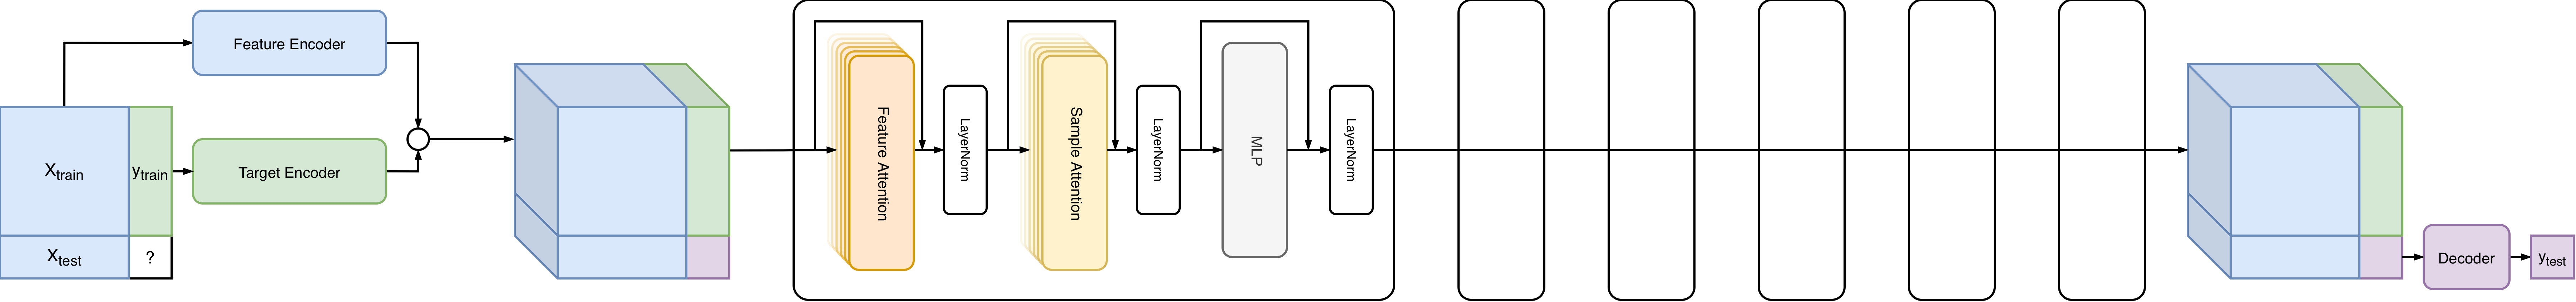
\includegraphics[width=\textwidth]{img/base-correct.png}
\end{frame}

\begin{frame}{TFM pretraining overview}
  \centering
  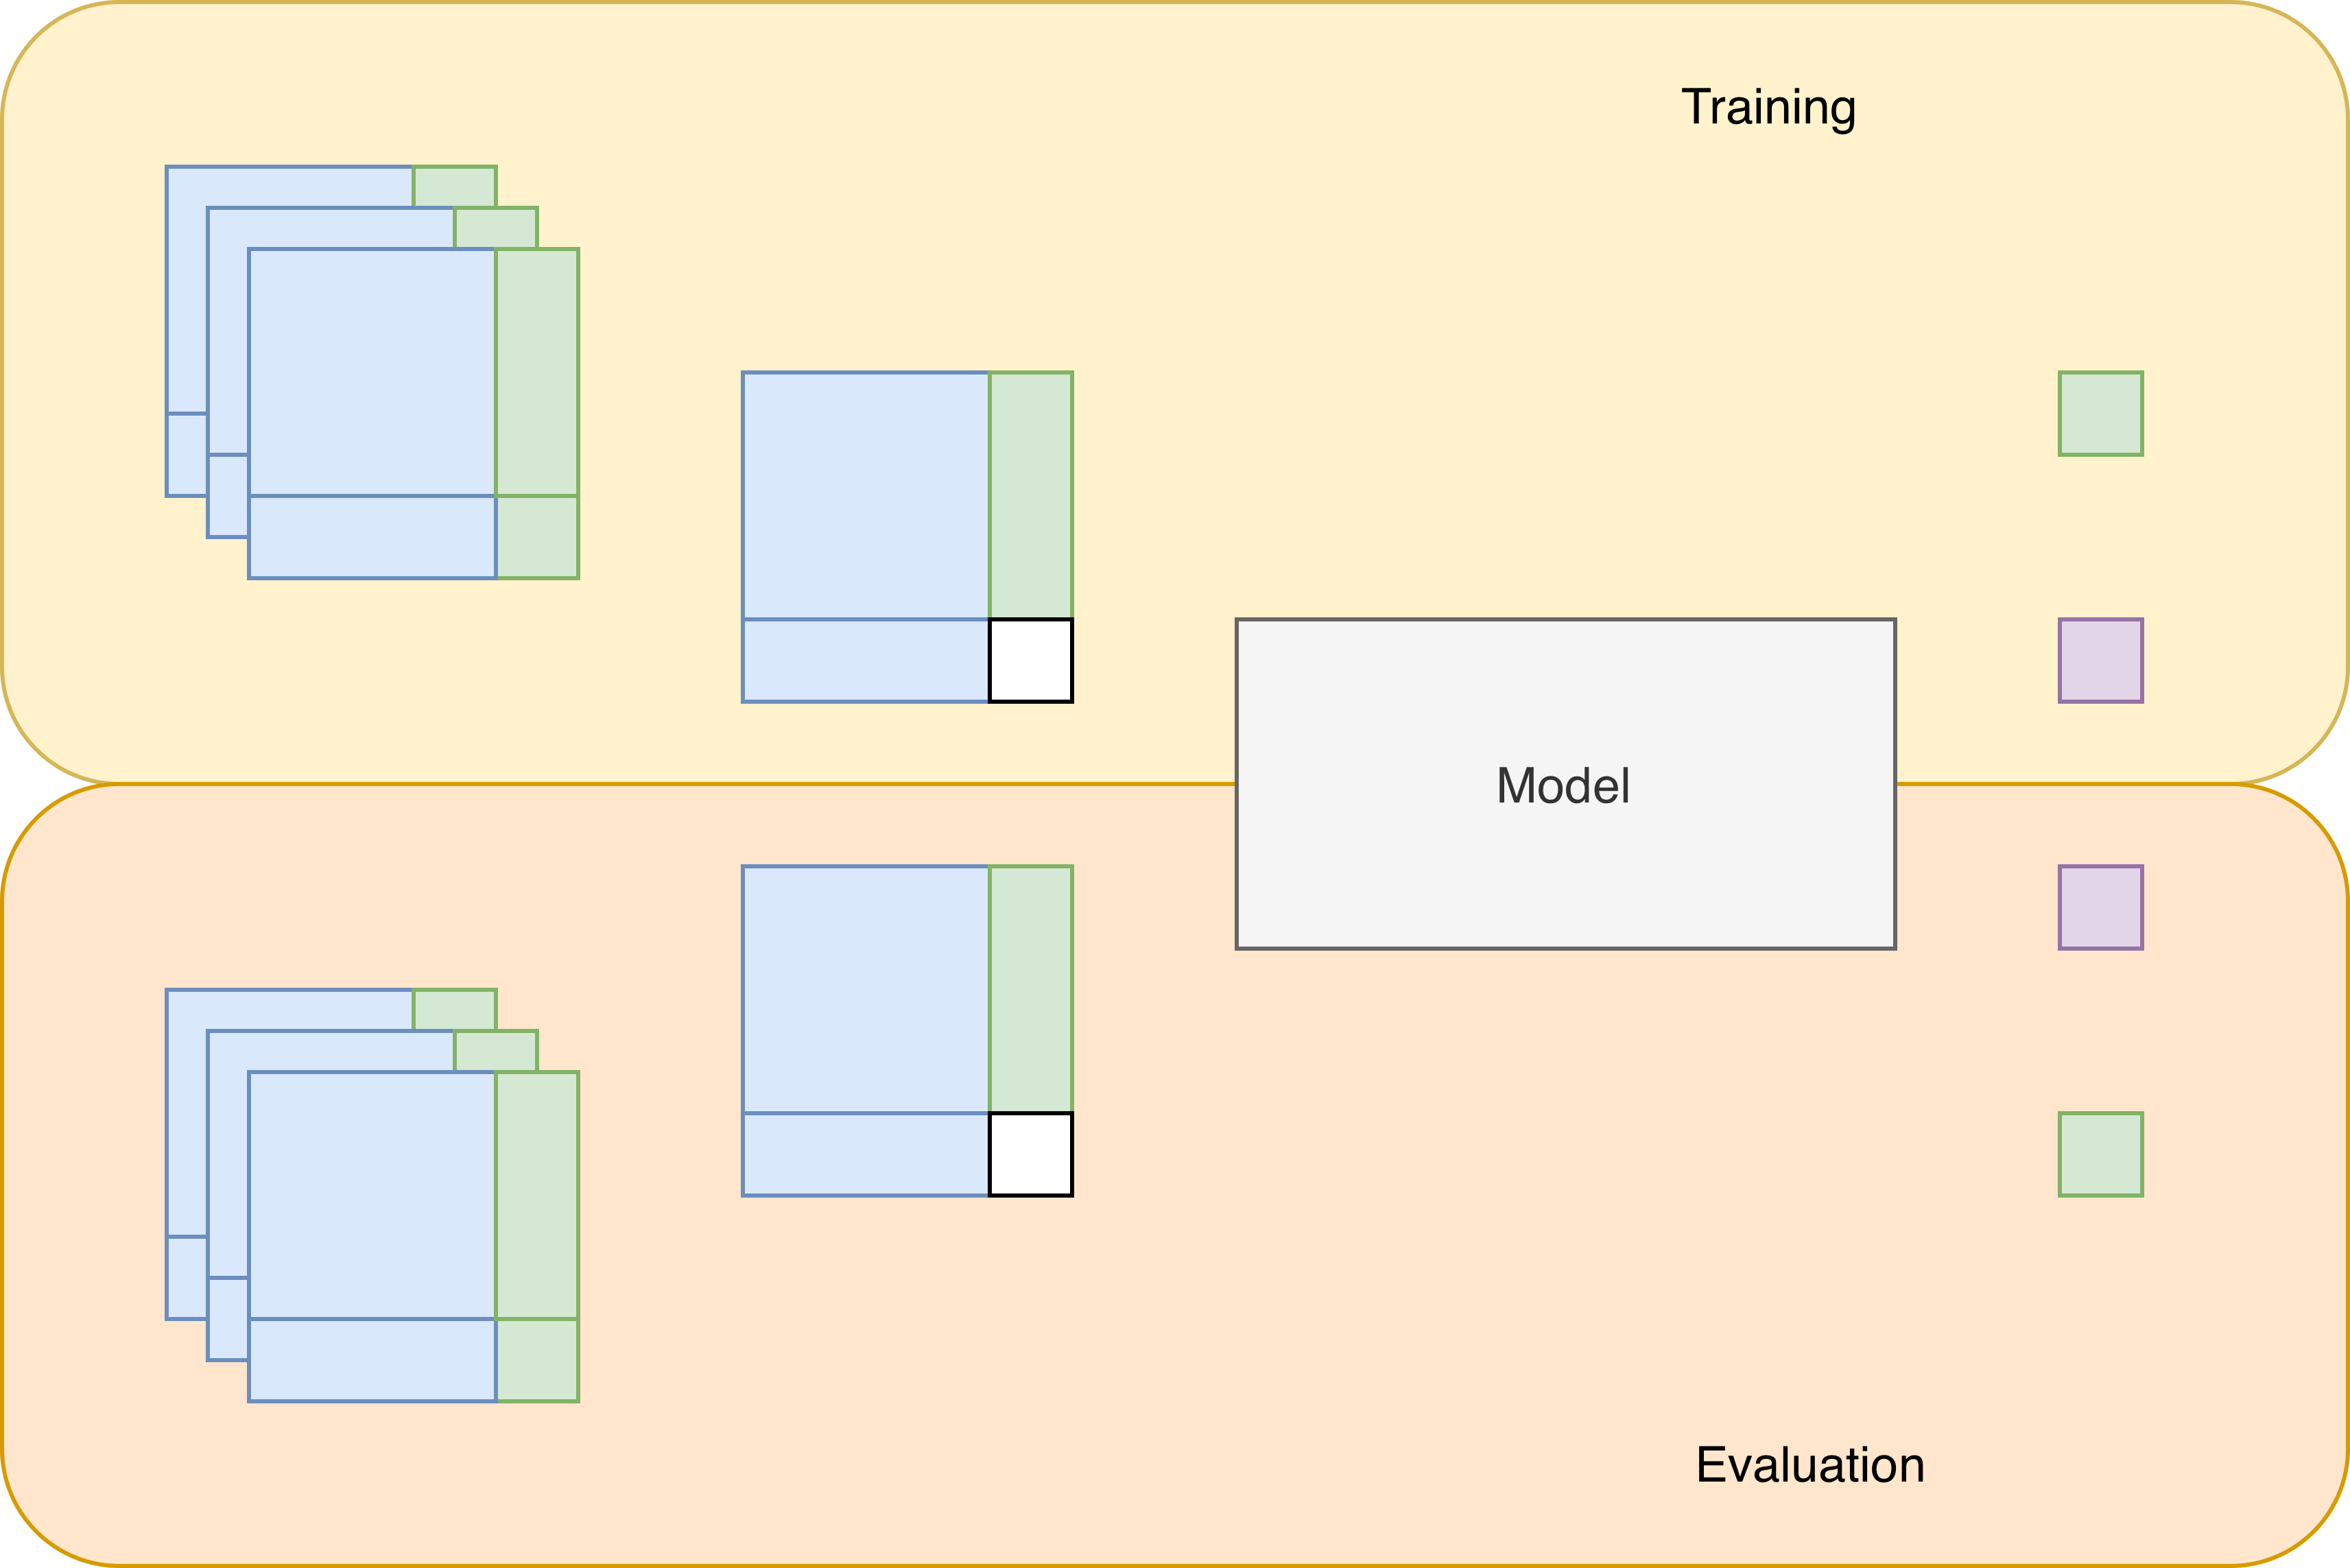
\includegraphics[height=0.82\textheight]{img/modded-loop.png}
\end{frame}

% ===========================================================================
\section{Record History}

\begin{frame}{Nine records: 74 minutes down to under one}
  \begin{columns}[c]
    \begin{column}{0.44\textwidth}
      \centering
      \begin{tikzpicture}
        \begin{axis}[
          width=\columnwidth, height=3.2cm,
          xlabel={Record \#}, ylabel={Wallclock (min)},
          ymode=log, log basis y={10},
          xtick={1,2,3,4,5,6,7,8,9},
          xmin=0.5, xmax=9.5, ymin=0.5, ymax=100,
          ytick={1,2,5,10,20,50,100},
          yticklabels={$1$,$2$,$5$,$10$,$20$,$50$,$100$},
          grid=both, grid style={lightgray!30, line width=0.3pt},
          tick style={black!60}, label style={font=\scriptsize}, tick label style={font=\tiny},
          every axis plot/.append style={mark=*, mark size=1.2pt, line width=0.6pt},
        ]
          \addplot+[
            color=accent,
            error bars/.cd, y dir=both, y explicit,
            error bar style={line width=0.4pt, accent!70},
          ] coordinates {
            (1, 74.32) +- (0, 0.90) (2, 54.41) +- (0, 0.29)
            (3, 10.10) +- (0, 1.52) (4,  9.26) +- (0, 1.07)
            (5,  7.57) +- (0, 0.93) (6,  3.88) +- (0, 0.68)
            (7,  3.48) +- (0, 0.30) (8,  2.15) +- (0, 0.52)
            (9,  0.92) +- (0, 0.04)
          };
        \end{axis}
      \end{tikzpicture}\\[1mm]
      \begin{tikzpicture}
        \begin{axis}[
          width=\columnwidth, height=3.2cm,
          xlabel={Record \#}, ylabel={Datasets seen},
          ymode=log, log basis y={10},
          xtick={1,2,3,4,5,6,7,8,9},
          xmin=0.5, xmax=9.5, ymin=2000, ymax=200000,
          ytick={2000,5000,10000,20000,50000,100000},
          yticklabels={$2$k,$5$k,$10$k,$20$k,$50$k,$100$k},
          grid=both, grid style={lightgray!30, line width=0.3pt},
          tick style={black!60}, label style={font=\scriptsize}, tick label style={font=\tiny},
          every axis plot/.append style={mark=*, mark size=1.2pt, line width=0.6pt},
        ]
          \addplot+[color=accent] coordinates {
            (1, 80576) (2, 45824) (3, 13184) (4, 13184)
            (5, 11200) (6,  9664) (7,  8768) (8,  4992) (9,  3648)
          };
        \end{axis}
      \end{tikzpicture}
    \end{column}
    \begin{column}{0.56\textwidth}
      \centering
      \scriptsize
      \setlength{\tabcolsep}{4pt}
      \begin{tabular}{@{}rrrl@{}}
        \toprule
        \# & Time (min) & Datasets & Technique \\
        \midrule
        1 & $74.32$ & $80{,}576$ & Baseline \\
        2 & $54.41$ & $45{,}824$ & Muon optimizer \\
        3 & $10.10$ & $13{,}184$ & SDPA, bf16, LR, width \\
        4 & $\phantom{0}9.26$ & $13{,}184$ & Batched Muon, compile \\
        5 & $\phantom{0}7.57$ & $11{,}200$ & Residual decay \\
        6 & $\phantom{0}3.88$ & $\phantom{0}9{,}664$ & RMSNorm, Thinking Rows \\
        7 & $\phantom{0}3.48$ & $\phantom{0}8{,}768$ & LAWA, AdamW WD \\
        8 & $\phantom{0}2.15$ & $\phantom{0}4{,}992$ & Repeated feature grouping \\
        9 & $\phantom{0}0.92$ & $\phantom{0}3{,}648$ & HPO, Muon WD, Mean-pool \\
        \bottomrule
      \end{tabular}
    \end{column}
  \end{columns}
\end{frame}

\begin{frame}{Record 1 --- Baseline \hfill \mut{74.32 min}}
  \begin{itemize}
    \item Taken from the TFM playground by me, merged into a single script.
  \end{itemize}
\end{frame}

\begin{frame}{Record 2 --- Muon optimizer \hfill \mut{54.41 min}}
  \begin{columns}[T]
    \begin{column}{0.6\textwidth}
      \begin{itemize}
        \item MomentUm Orthogonalized by Newton--Schulz
        \begin{itemize}
          \item 2D hidden matrices $\to Muon$
        \end{itemize}
        \medskip
        \item Orthogonalize the momentum
        \begin{itemize}
          \item rebalances rare-but-important directions
        \end{itemize}
        \medskip
        \item Slower per step but fewer steps
        \item General optimizer, carries over from LLMs and CV(CIFAR-10)
      \end{itemize}
    \end{column}
    \begin{column}{0.4\textwidth}
      \centering
      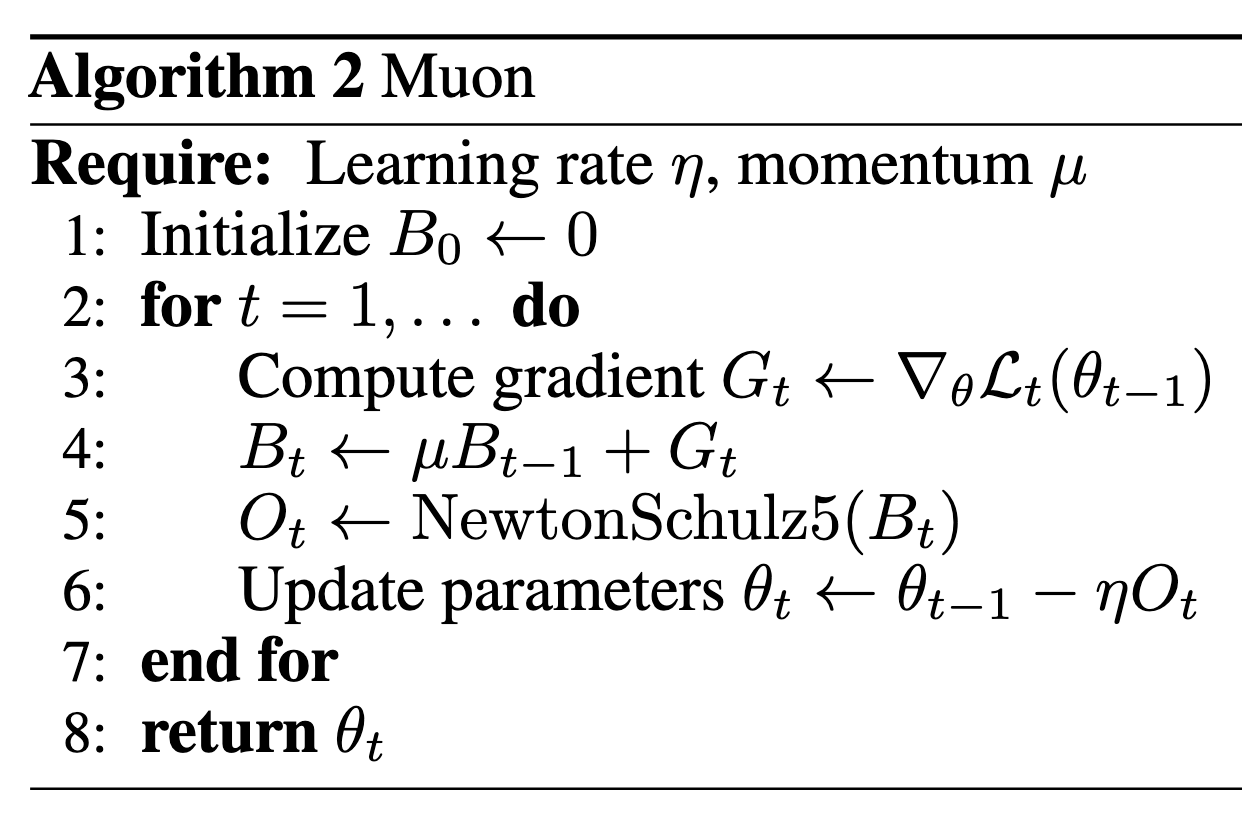
\includegraphics[width=\textwidth]{img/muon-algo.png}
      \cit{Jordan '24}
    \end{column}
  \end{columns}
\end{frame}

\begin{frame}{Record 3 --- SDPA, bf16, LR, width \hfill \mut{10.10 min}}
  \begin{itemize}
    \item LR $10^{-4} \to 10^{-3}$
    \item Explicit-QKV SDPA rewrite (fused attention), also moves post-norm to pre-norm
    \item Embedding $192 \to 256$, heads $6 \to 4$
    \item bf16 autocast (train + eval) + TF32 matmul
  \end{itemize}
  \vfill
  \mut{\footnotesize by @carterprince}
\end{frame}

\begin{frame}{Record 4 --- Batched Muon \& compile \hfill \mut{9.26 min}}
  \begin{itemize}
    \item QKV
    \begin{itemize}
      \item Before: orthogonalize the 3 in a Python loop
      \item Now: batched (3, e, e) Newton-Schulz, all 3 in one kernel
    \end{itemize}
    \item torch.compile on the transformer block forward
  \end{itemize}
  \vfill
  \mut{\footnotesize by @carterprince}
\end{frame}

\begin{frame}{Record 5 --- Residual decay \hfill \mut{7.57 min}}
  \centering
  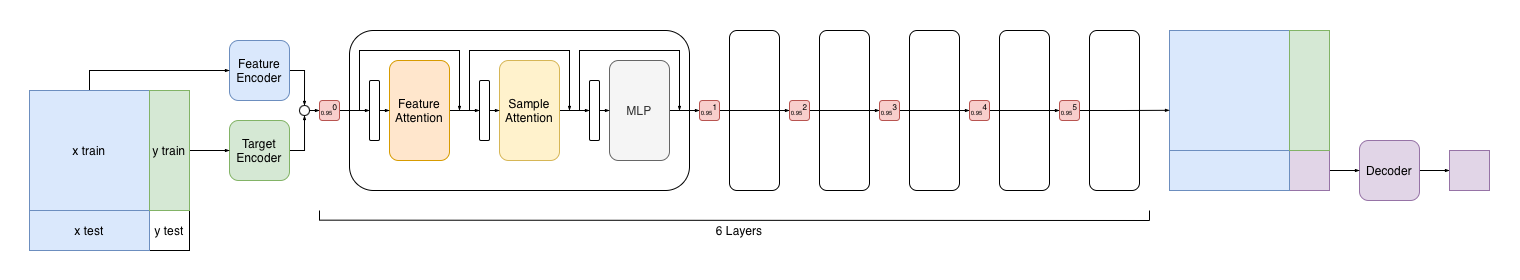
\includegraphics[width=\textwidth]{img/residual-decay-diagram.png}
  \begin{itemize}
    \item Scale the residual stream entering layer $i$ by $0.95^i$
    \item Fixed base $0.95$, exponential in depth
  \end{itemize}
\end{frame}

\begin{frame}{Record 6 --- RMSNorm \& Thinking rows \hfill \mut{3.88 min}}
  \centering
  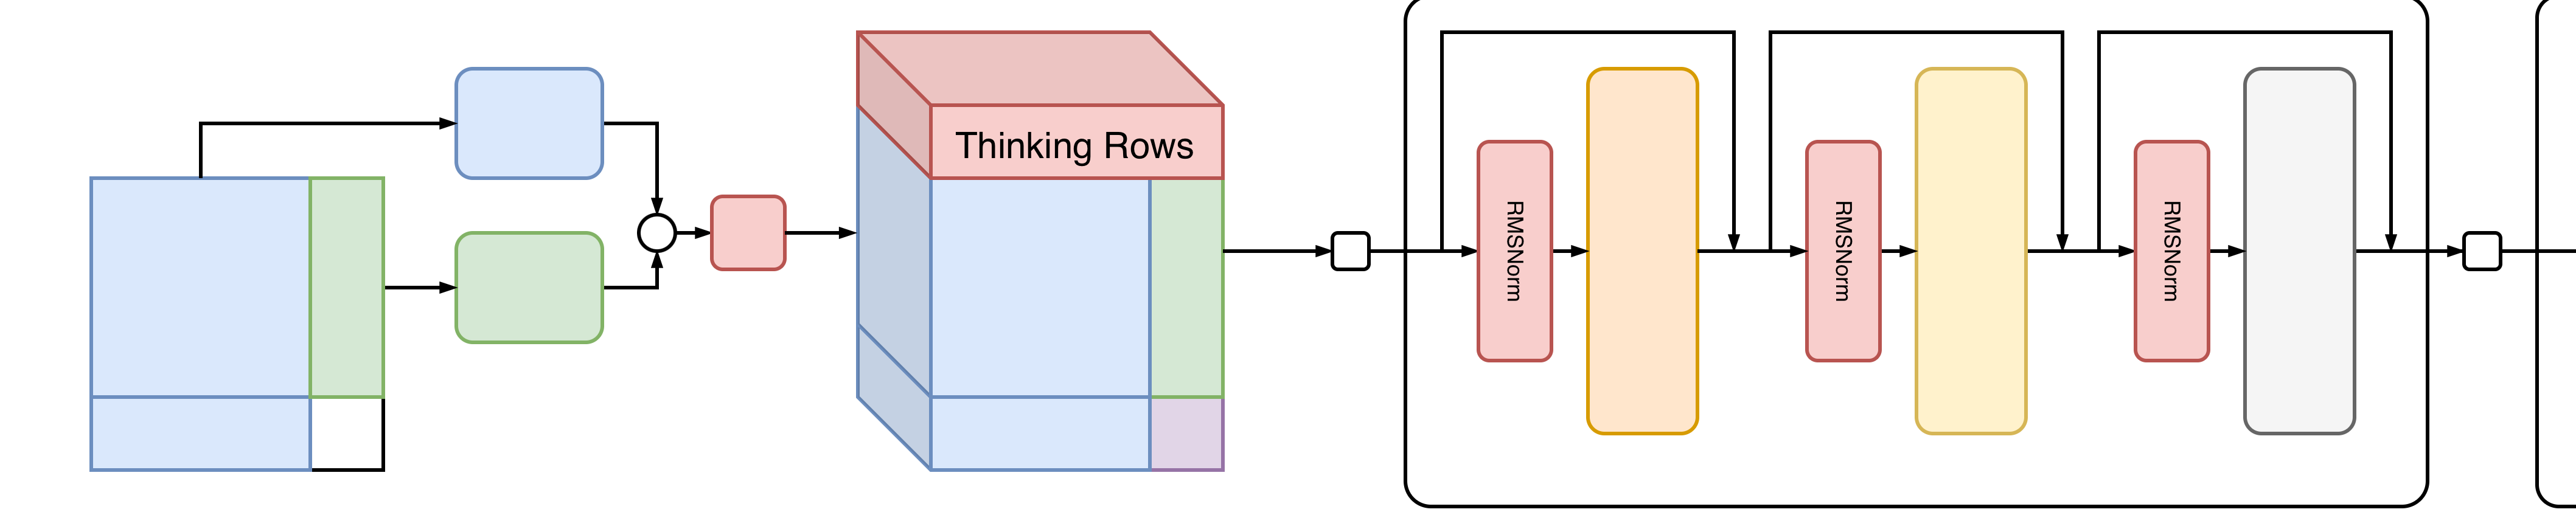
\includegraphics[width=\textwidth]{img/rmsthink-diagram-crop.png}
  \begin{itemize}
    \item LowerPrecisionRMSNorm: replace the LayerNorms, skip the fp32 upcast \cit{TabPFNv2.6}
    \item Thinking rows: prepend 16 learnable row tokens \cit{TabPFNv2.5}
    \item Thinking rows drive most of the gain
  \end{itemize}
\end{frame}

\begin{frame}{Record 7 --- LAWA \& AdamW weight decay \hfill \mut{3.48 min}}
  \begin{itemize}
    \item LAWA: \cit{Kaddour '22 / Sanyal '23}
    \begin{itemize}
      \item average the last K=10 epoch checkpoints for eval
      \item keep the training weights
    \end{itemize}
    \item AdamW weight decay 0.01
  \end{itemize}
\end{frame}

\begin{frame}{Record 8 --- Repeated feature grouping \hfill \mut{2.15 min}}
  \centering
  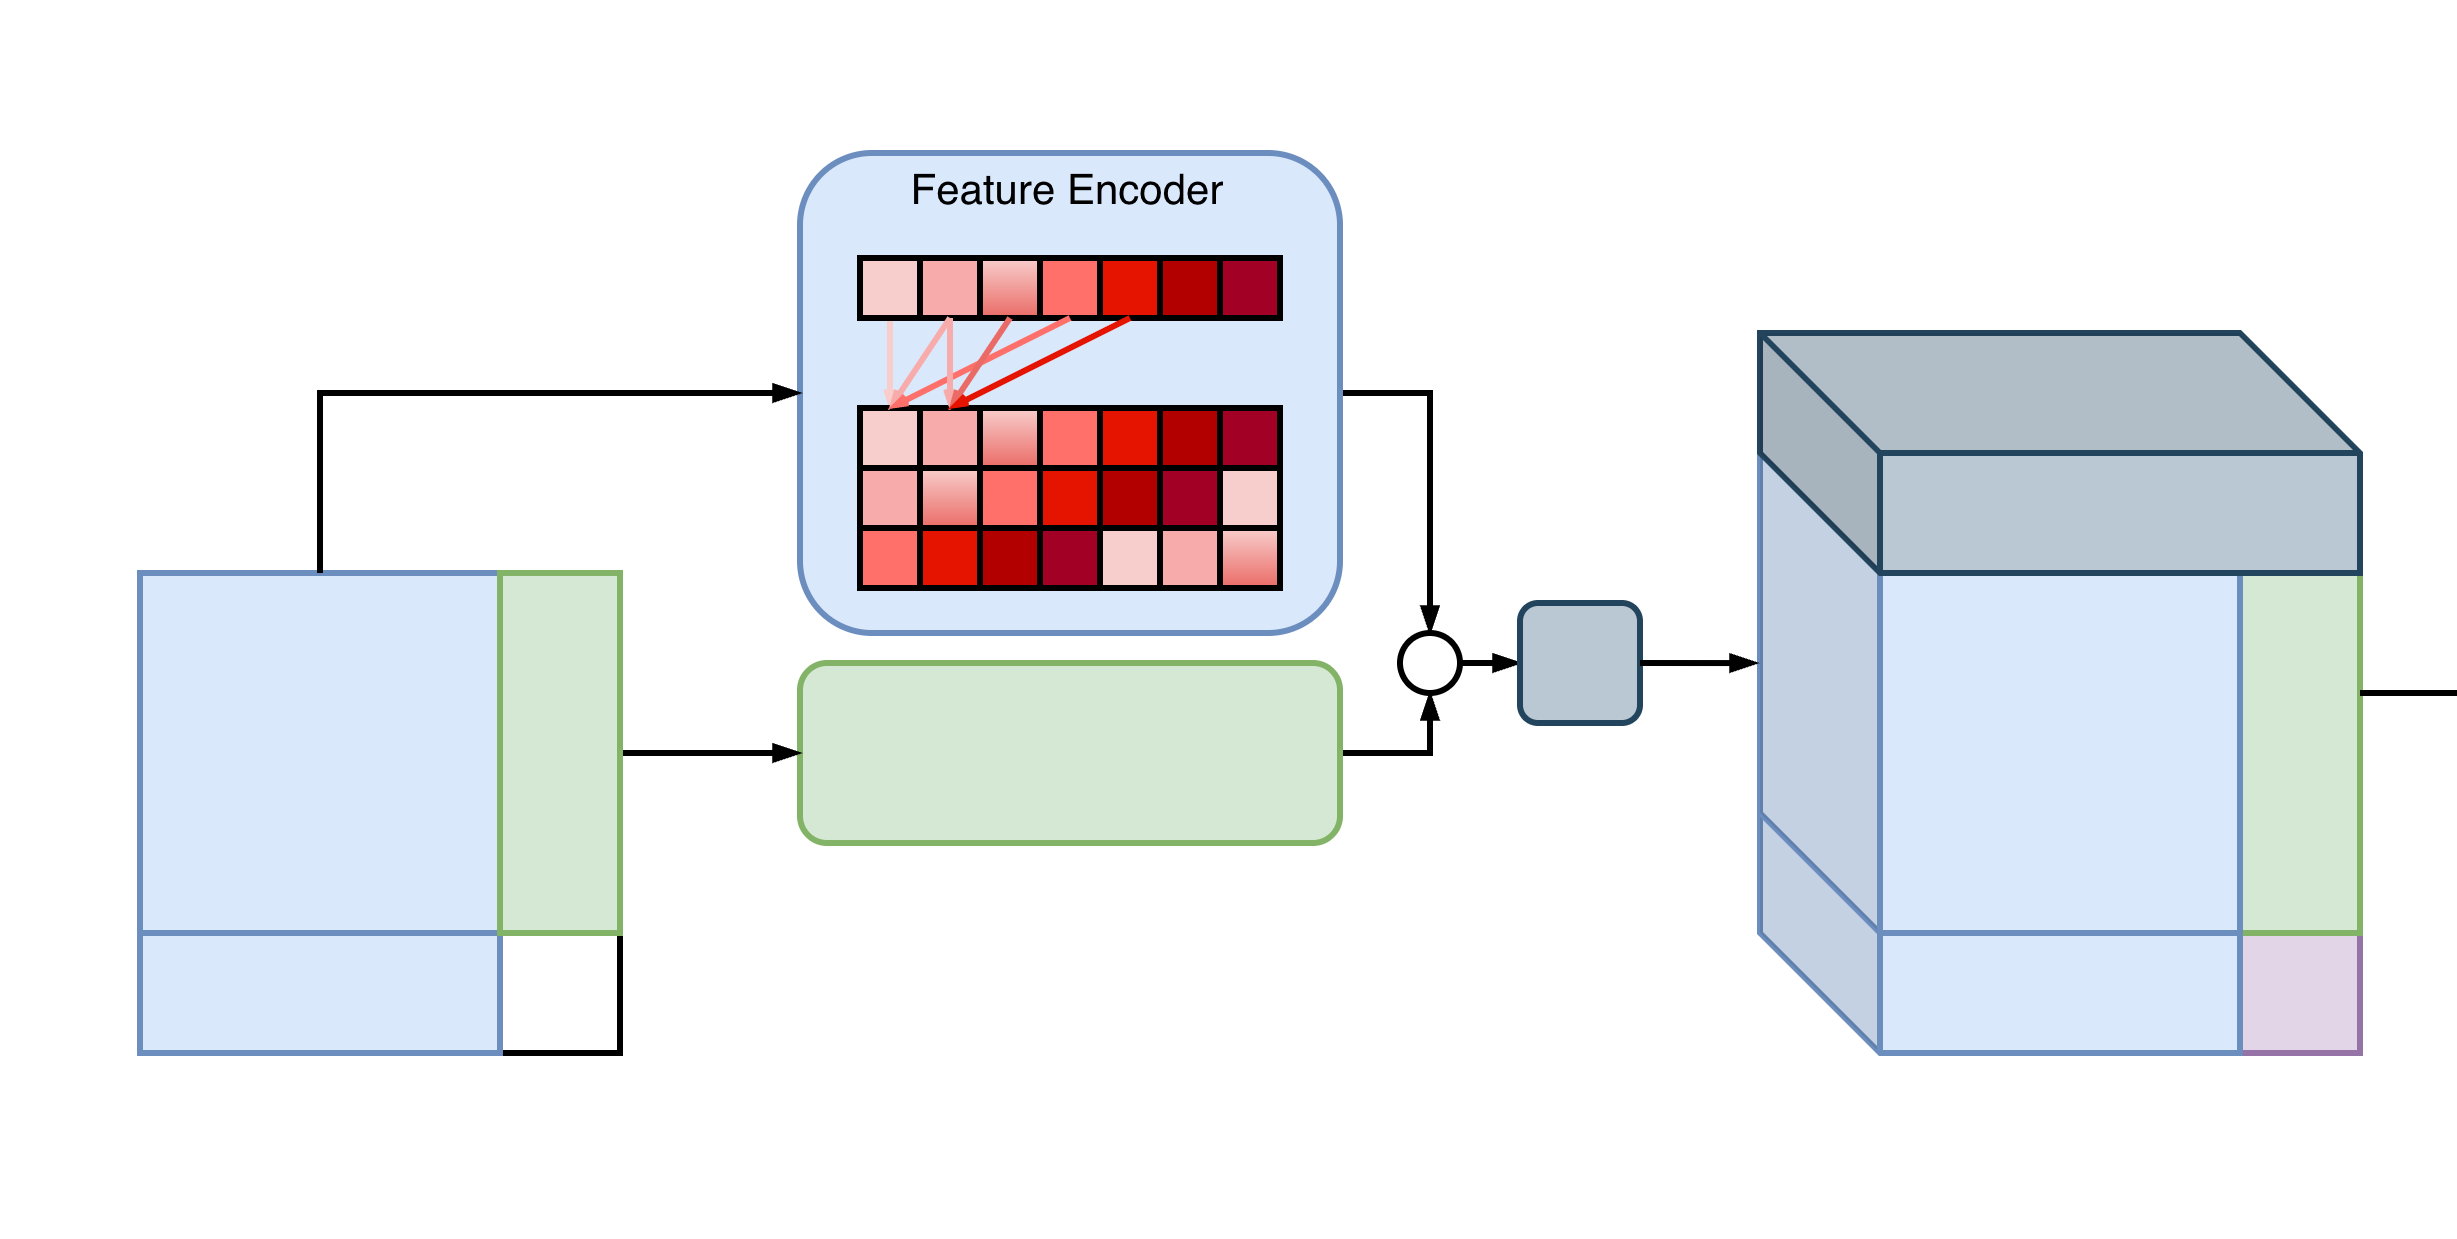
\includegraphics[width=0.62\textwidth]{img/feature-group-diagram.png}
  \begin{itemize}
    \item Before: embed each feature alone, Linear(1, e)
    \item Now: embed each as a triplet $(x_j, x_{j+1}, x_{j+3})$, Linear(3, e)
    \item Prevents representation collapse on similar features \cit{TabICLv2}
  \end{itemize}
\end{frame}

\begin{frame}{Record 9 --- Autoresearch HPO, Muon WD, Mean-pool decoder \hfill \mut{0.92 min}}
  \begin{itemize}
    \item Found with autoresearch \cit{Karpathy '26}:
    \begin{itemize}
      \item LLM-driven HPO + architecture search
      \item with human intervention
    \end{itemize}
    \item HPO: 7 knobs tuned (layers most impactful)
    \item Muon weight decay 0.1
    \item Mean-pool decoder: mean over feature tokens at test rows, not the target token
  \end{itemize}
\end{frame}

\begin{frame}{Convergence to target over time}
  \centering
  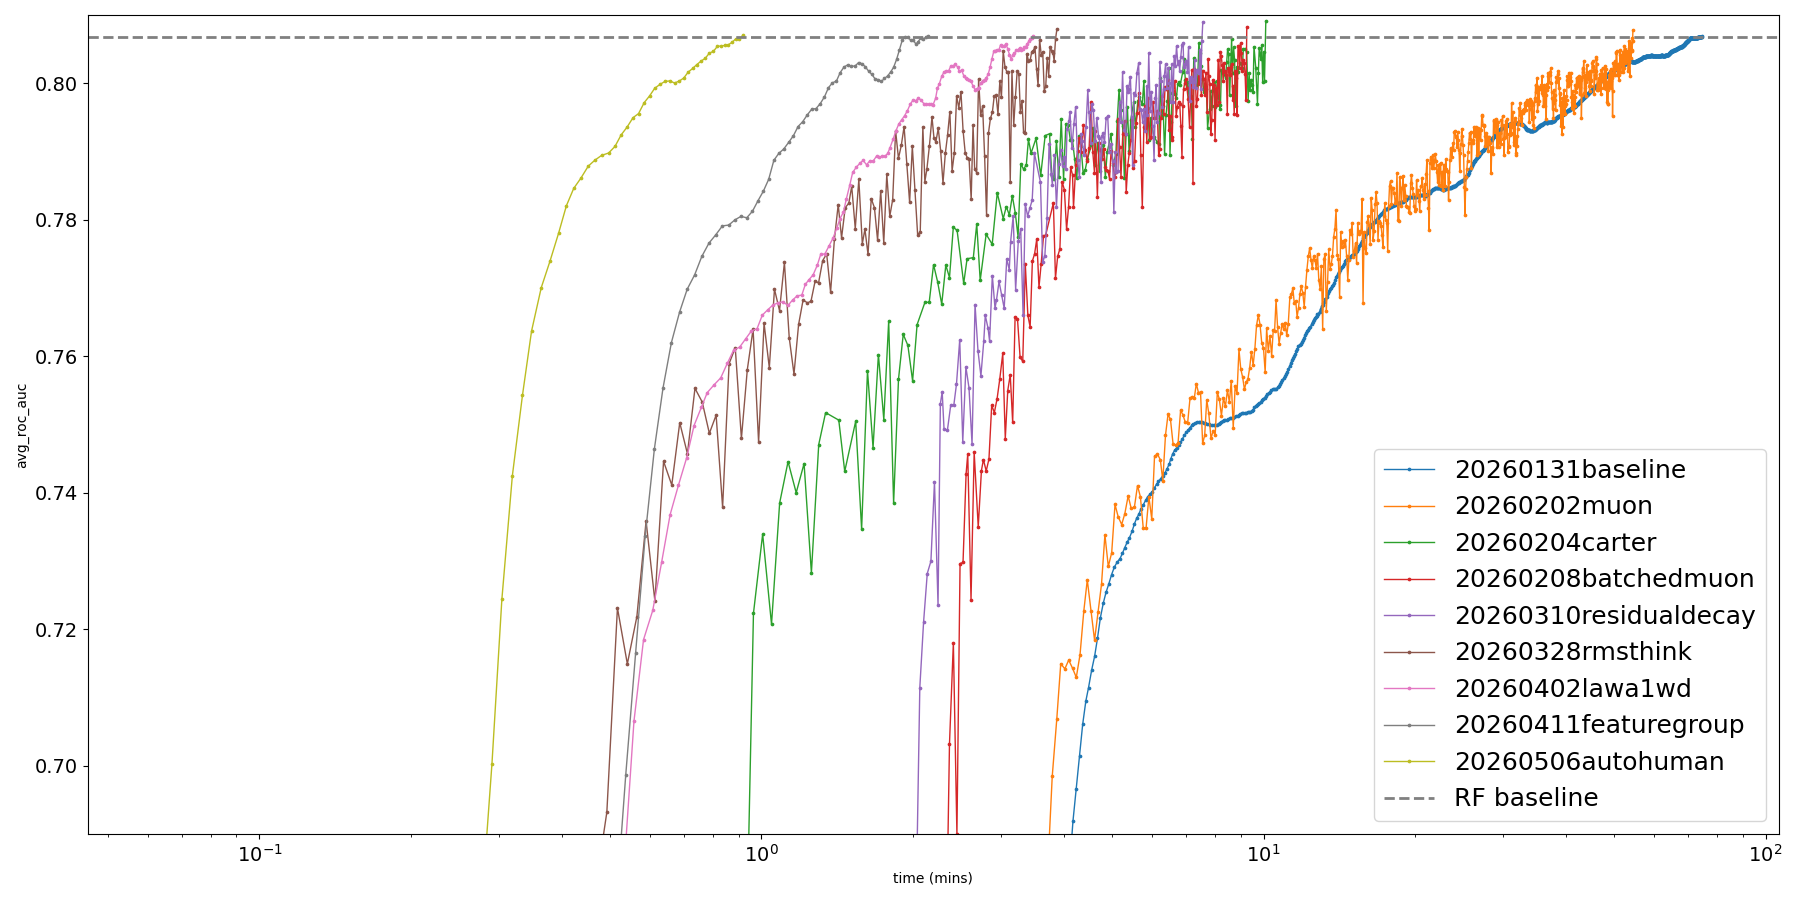
\includegraphics[width=0.9\textwidth]{img/records-time.png}
\end{frame}

% ===========================================================================
\section{Where We Landed}

\begin{frame}{The modded architecture}
  \centering
  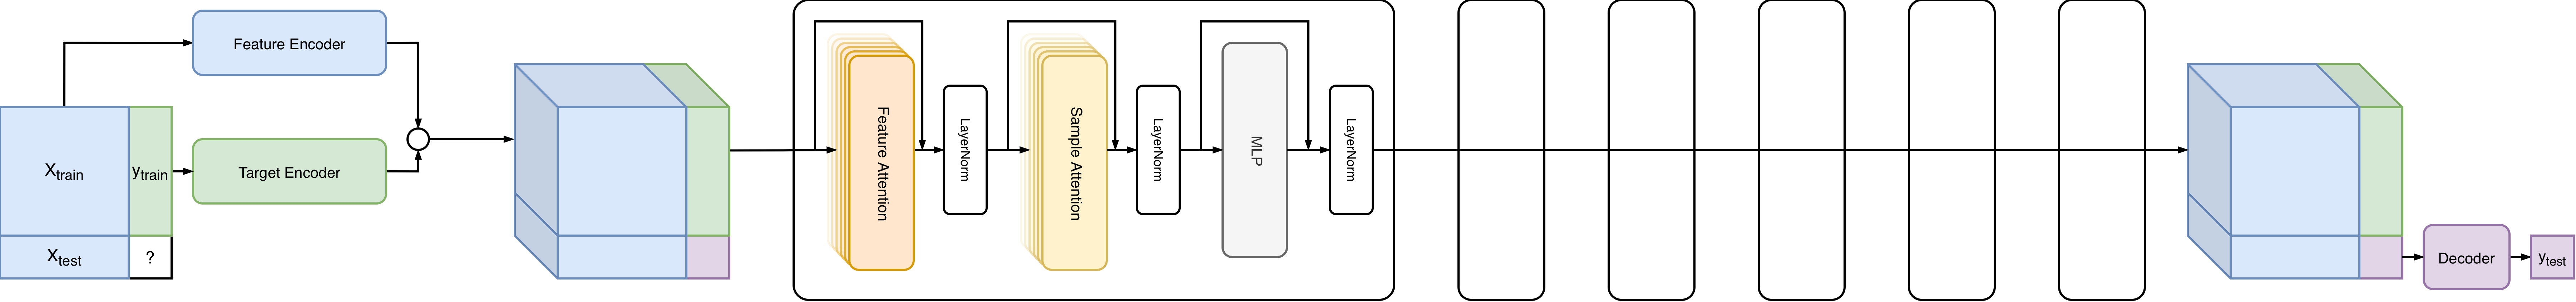
\includegraphics[width=\textwidth]{img/base-correct.png}\\[3mm]
  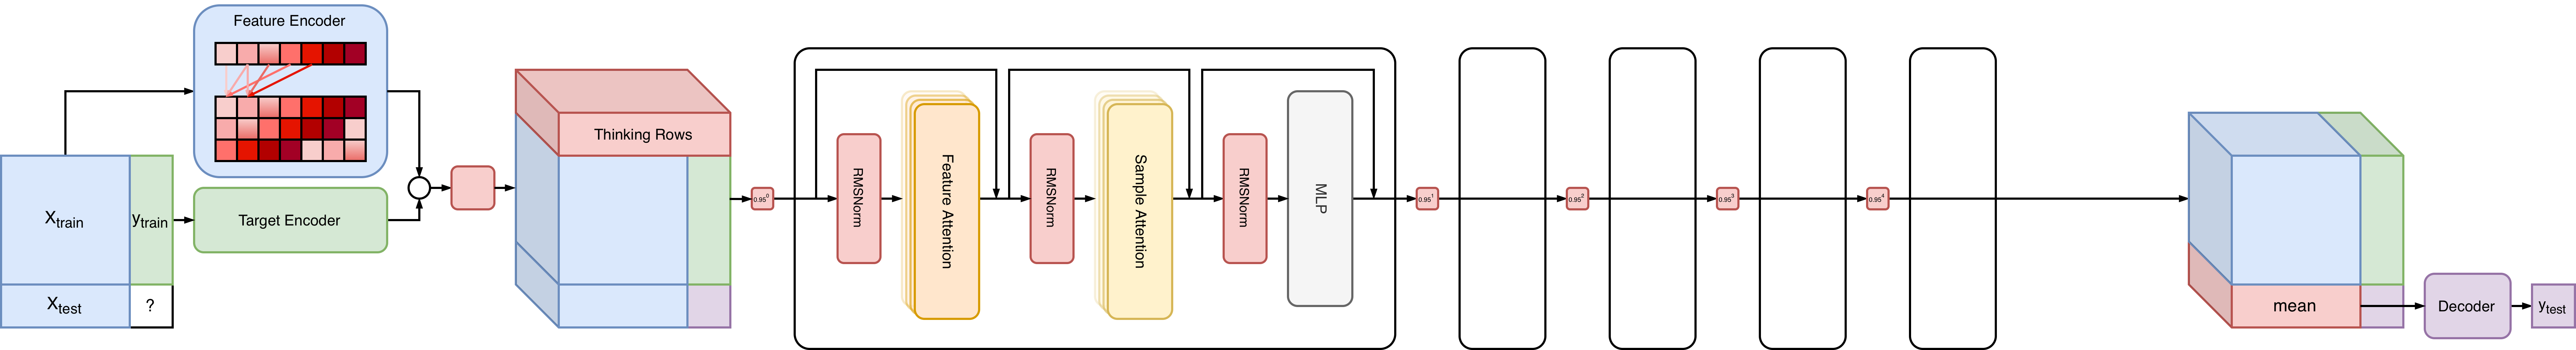
\includegraphics[width=\textwidth]{img/modded.png}
\end{frame}

\begin{frame}{Baseline vs.\ modded}
  \footnotesize
  \begin{columns}[T]
    \begin{column}{0.5\textwidth}
      \textit{Architecture}
      \begin{tabular}{@{}lll@{}}
        \toprule
                       & Baseline & Modded \\
        \midrule
        Layers         & 6 & 5 \\
        Heads          & 6 & 4 \\
        Embedding      & 192 & 256 \\
        Norm           & post-LN & pre-RMSNorm \\
        Feat.\ group   & 1 & 5 \\
        Thinking rows  & 0 & 24 \\
        Residual decay & 1.0 & 0.95 \\
        Decoder in     & target & mean feats \\
        \bottomrule
      \end{tabular}
    \end{column}
    \begin{column}{0.5\textwidth}
      \textit{Optimization \& throughput}
      \begin{tabular}{@{}lll@{}}
        \toprule
                       & Baseline & Modded \\
        \midrule
        Optimizer      & sf-AdamW & sf-AdamW+Muon \\
        LR             & $10^{-4}$ & $10^{-3}$ \\
        AdamW WD       & 0 & 0.01 \\
        Muon mom.      & -- & 0.96 \\
        Muon WD        & -- & 0.1 \\
        Grad clip      & 1.0 & 2.0 \\
        LAWA           & -- & $K{=}10$ \\
        Batch size     & 1 & 2 \\
        Precision      & fp32 & bf16 \\
        \bottomrule
      \end{tabular}
    \end{column}
  \end{columns}
\end{frame}

\begin{frame}{Beyond the target: what if we keep training?}
  \centering
  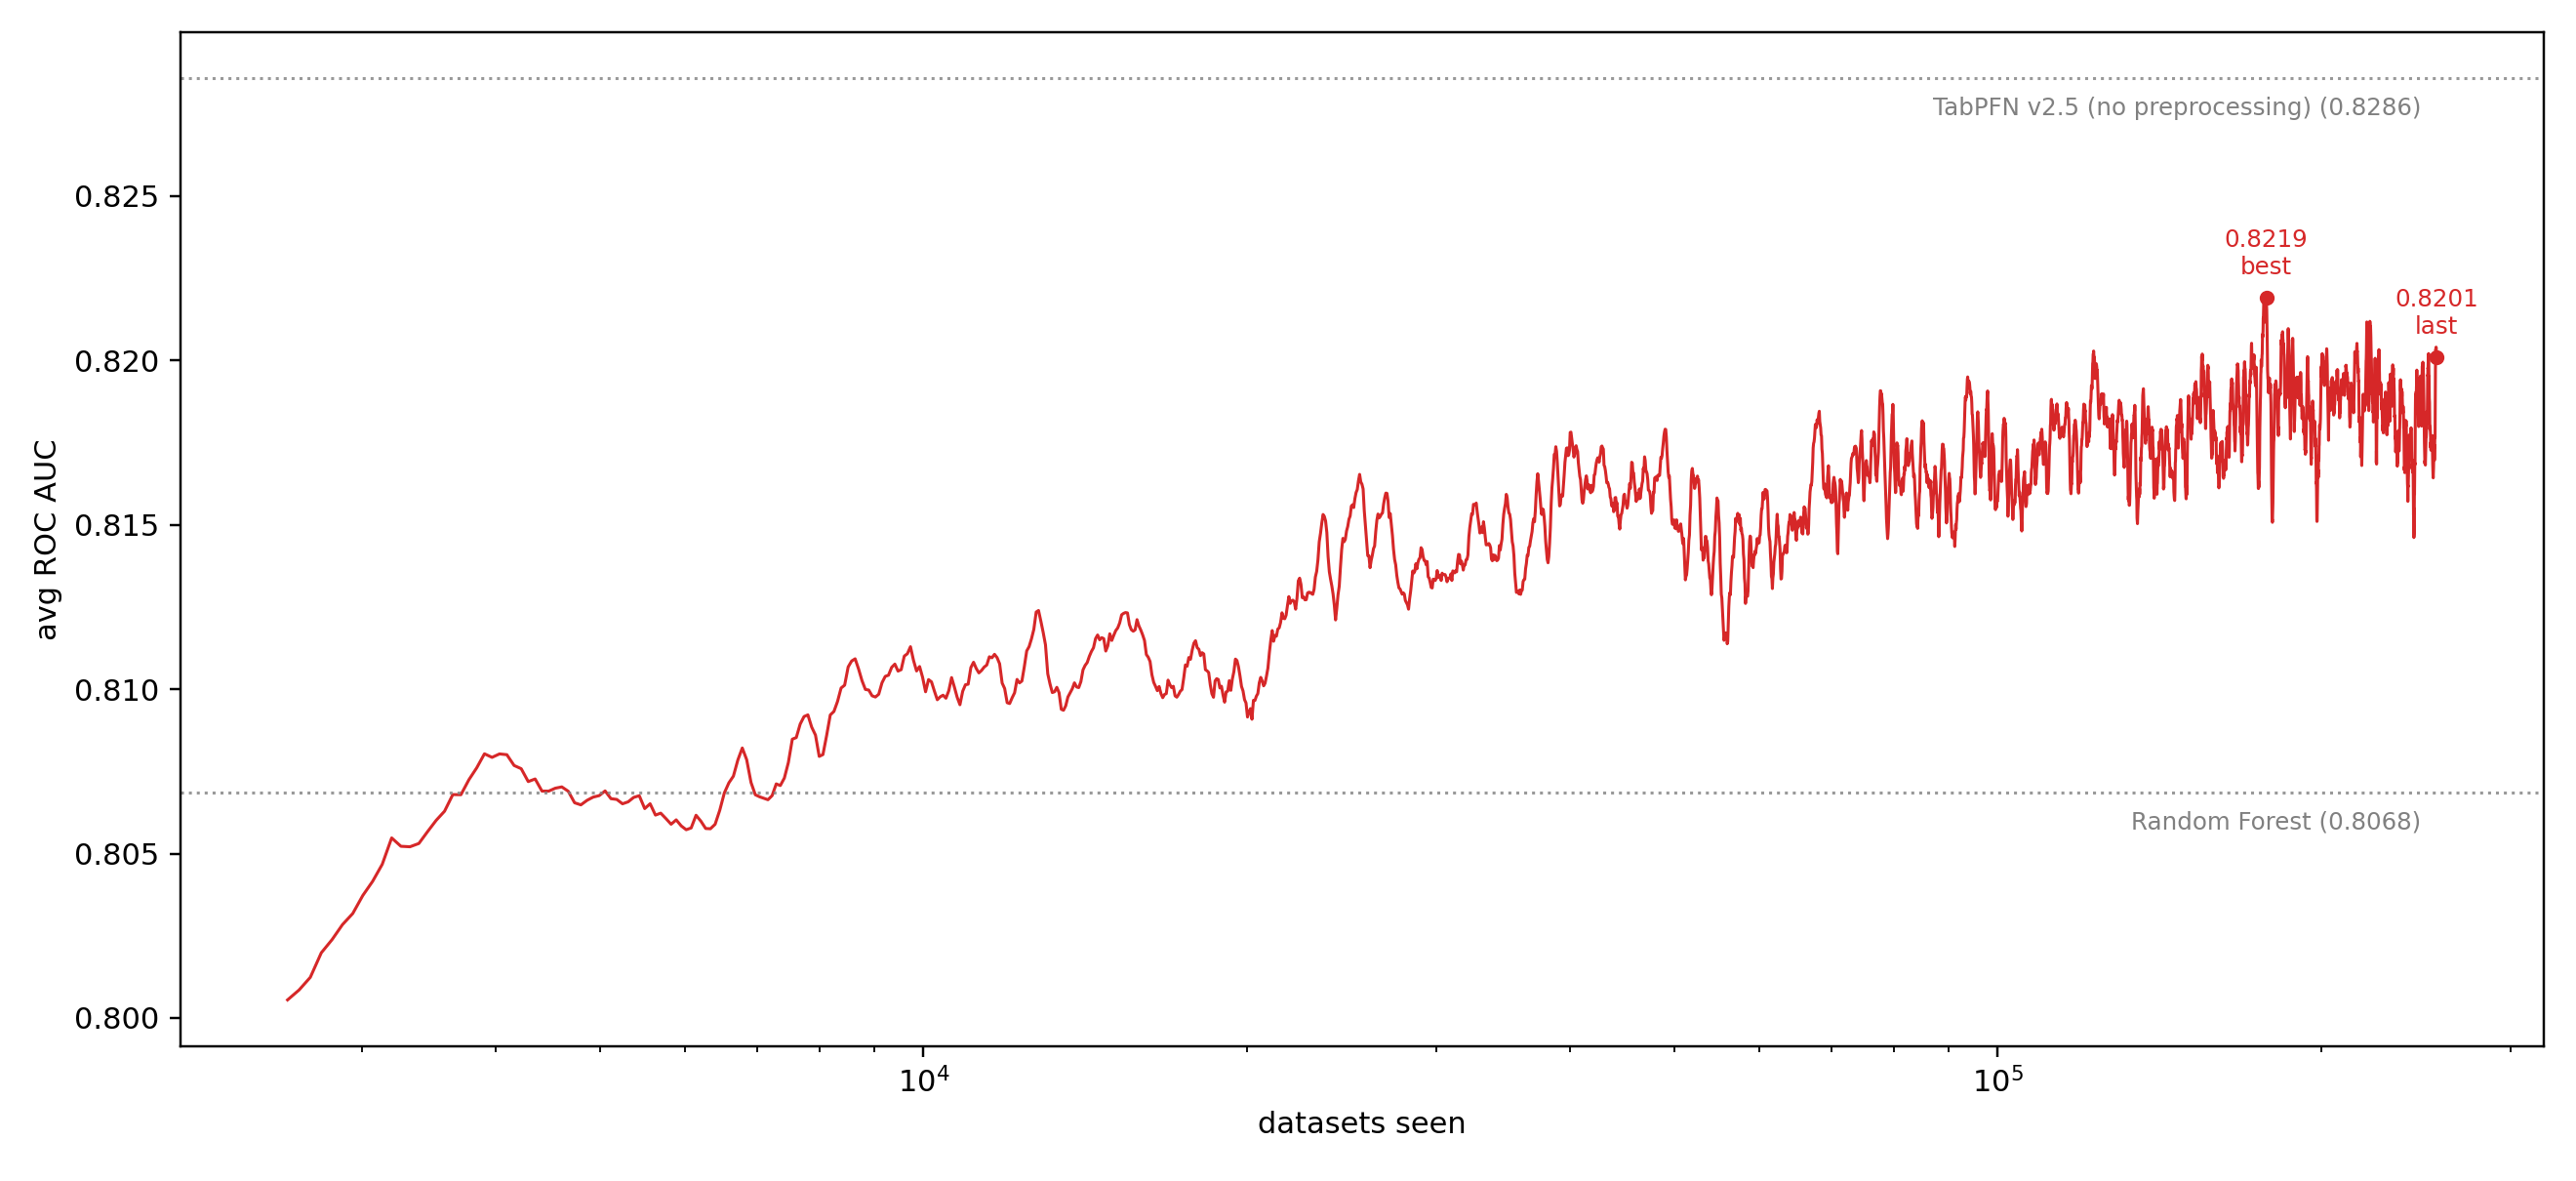
\includegraphics[width=0.88\textwidth]{img/longrun.png}
\end{frame}

\begin{frame}{Does it only work on TabArena?}
  No --- the same record ladder holds on the TabPFN-paper eval tasks.
  \centering
  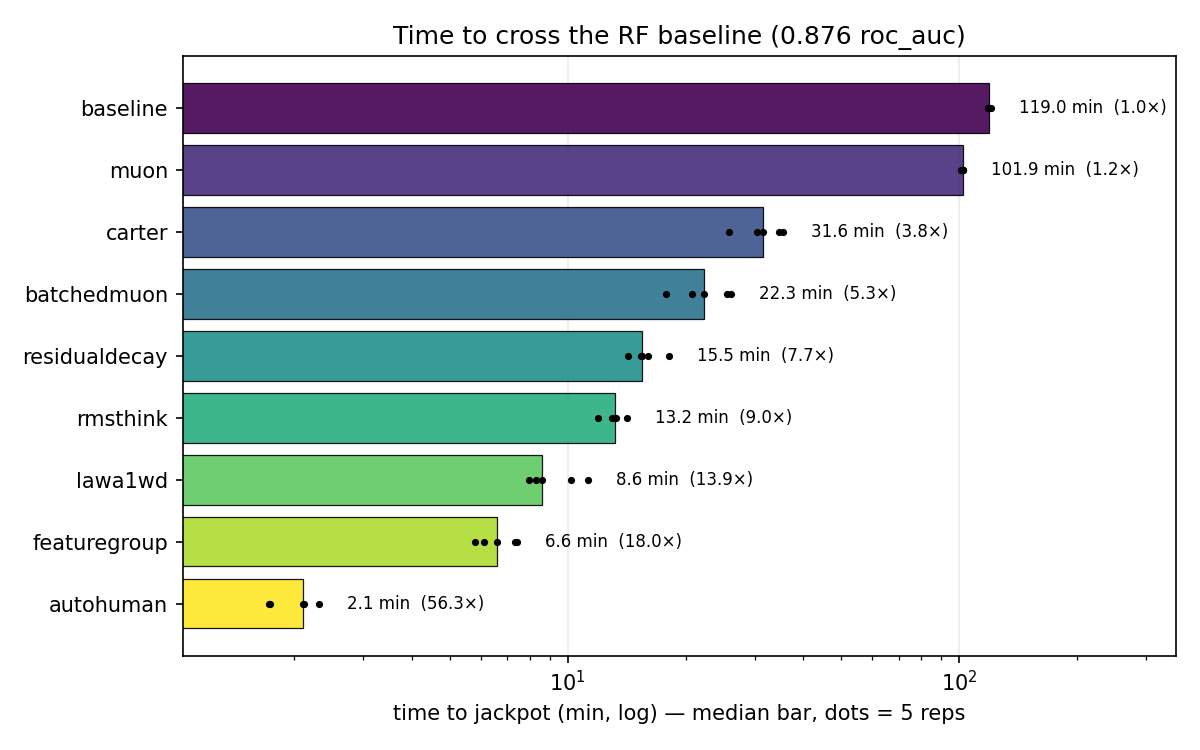
\includegraphics[width=0.72\textwidth]{img/ttj-tabpfn.png}
\end{frame}

\begin{frame}{Time to jackpot --- records vs.\ retime}
  \begin{columns}[c]
    \begin{column}{0.5\textwidth}
      \centering
      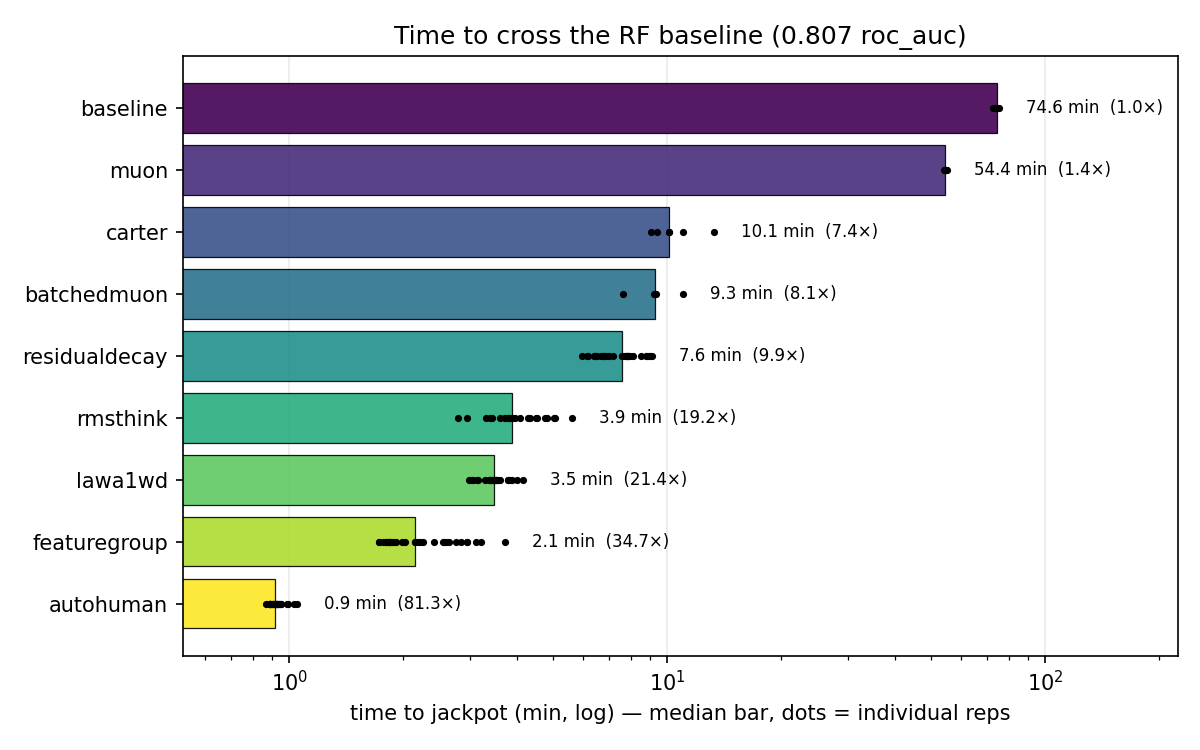
\includegraphics[width=\textwidth]{img/ttj-records.png}\\
      \mut{\footnotesize record times}
    \end{column}
    \begin{column}{0.5\textwidth}
      \centering
      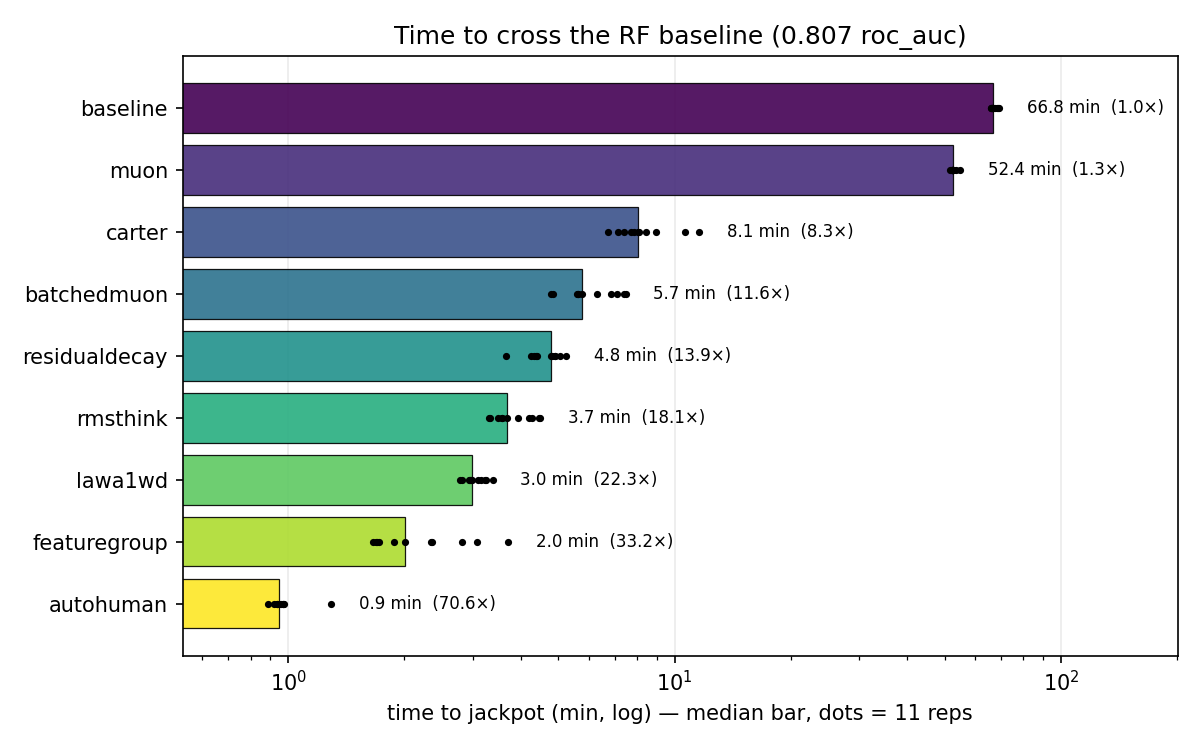
\includegraphics[width=\textwidth]{img/ttj-retime.png}\\
      \mut{\footnotesize controlled re-run, 11 reps}
    \end{column}
  \end{columns}
\end{frame}

\begin{frame}{Conclusion}
  \begin{itemize}
    \item An open speedrun for tabular foundation model pretraining, built on nanoTabPFN
    \item 60--80$\times$ faster pretraining to the same targets
    \item The same recipe keeps improving past the targets when given a longer budget
    \item The speedrun itself is the contribution:
    \begin{itemize}
      \item a protocol to add, verify, and stack improvements
    \end{itemize}
  \end{itemize}
\end{frame}

\begin{frame}{Limitations}
  \begin{itemize}
    \item No full leave-one-out ablation of the final record\\
      \mut{not every component is claimed independently beneficial}
      \mut{, stacking effect is real}
    \item Classification only
    \item Subsampled evaluation
    \item Single hardware: 1$\times$L40S
  \end{itemize}
\end{frame}

\begin{frame}{Future work}
  \begin{itemize}
    \item Prior not touched (not really true)
    \begin{itemize}
      \item Prior track
    \end{itemize}
    \item Autoresearch
    \begin{itemize}
      \item Giving agents access to more training info
    \end{itemize}
    \item There is no end to this speedrun \emoji{rocket} (still open to submissions)
  \end{itemize}
\end{frame}

\begin{frame}{GitHub}
  \centering
  
\includegraphics[width=0.85\textwidth]{img/modded-github.png}
  \\[4mm]
  \href{https://github.com/borawhocodess/modded-nanotabpfn}{\hl{github.com/borawhocodess/modded-nanotabpfn}}
\end{frame}

\begin{frame}{Paper}
  \centering
  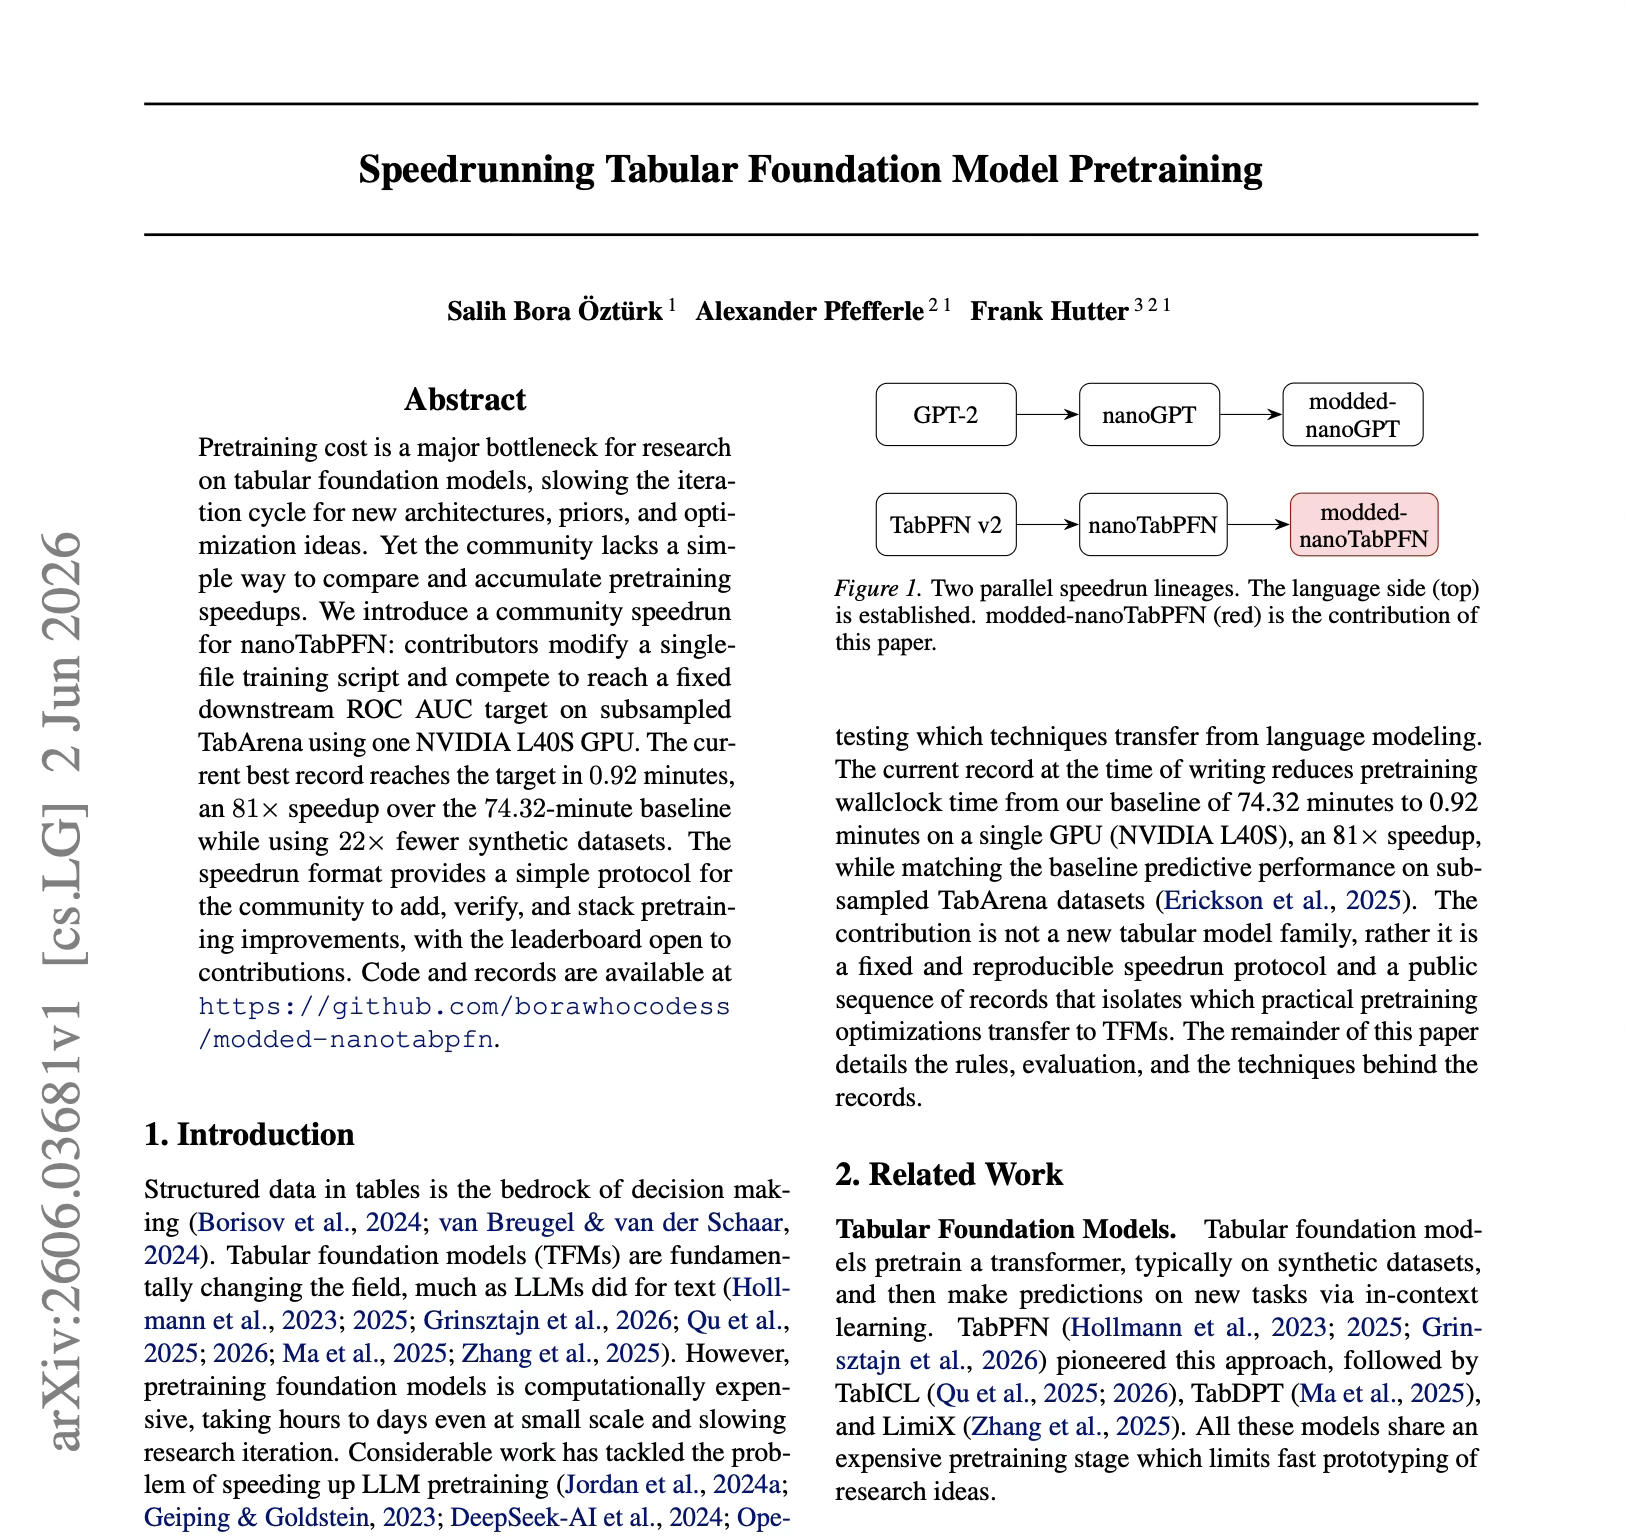
\includegraphics[height=6cm]{img/modded-paper.png}
  \\[3mm]
  \href{https://arxiv.org/abs/2606.03681}{\hl{arxiv.org/abs/2606.03681}}
  \\[1mm]
  \mut{accepted at the FM4SD workshop @ ICML 2026}
\end{frame}

% ===========================================================================
\begin{frame}[standout]
  Thank you \quad$\cdot$\quad Questions welcome
\end{frame}

% ===========================================================================
\appendix

\begin{frame}{Other Competition examples}
  \begin{itemize}
    \item \href{https://github.com/KellerJordan/modded-nanogpt}{\hl{modded-nanogpt --- speedrun}}\\
      \mut{NanoGPT to a fixed loss target, minimize wallclock --- the original}
    \smallskip
    \item \href{https://github.com/KellerJordan/modded-nanogpt/tree/master/records/track_3_optimization}{\hl{modded-nanogpt --- optimizer track}}\\
      \mut{minimize \emph{step count}, not wallclock --- slow-but-efficient optimizers welcome}
    \smallskip
    \item \href{https://github.com/qlabs-eng/slowrun}{\hl{qlabs-eng/slowrun}}\\
      \mut{100M tokens, infinite compute --- lowest val loss wins}
    \smallskip
    \item \href{https://github.com/openai/parameter-golf}{\hl{openai/parameter-golf}}\\
      \mut{best language model that fits in a 16\,MB artifact, trains in under 10 min}
    \smallskip
    \item \href{https://github.com/anadim/AdderBoard}{\hl{anadim/AdderBoard}}\\
      \mut{smallest transformer that adds two 10-digit numbers --- winners at 6 and 36 params}
  \end{itemize}
\end{frame}

\begin{frame}{Backup --- Record 3 ablation \hfill \mut{\footnotesize 5 reps per knob, median min}}
  \footnotesize
  \begin{columns}[T]
    \begin{column}{0.5\textwidth}
      \centering
      \textit{Add each knob to Muon} \mut{(54.41)}
      \begin{tabular}{@{}lrr@{}}
        \toprule
        knob & median & $\Delta$ \\
        \midrule
        LR                & $31.52$ & $-42\%$ \\
        explicit-QKV SDPA & $38.99$ & $-28\%$ \\
        matmul high (TF32)& $45.06$ & $-17\%$ \\
        embed, heads      & $45.78$ & $-16\%$ \\
        autocast eval     & $49.13$ & $-10\%$ \\
        autocast train    & $49.31$ & $\phantom{0}-9\%$ \\
        \bottomrule
      \end{tabular}
    \end{column}
    \begin{column}{0.5\textwidth}
      \centering
      \textit{Remove each knob from record} \mut{(10.10)}
      \begin{tabular}{@{}lrr@{}}
        \toprule
        knob & median & $\Delta$ \\
        \midrule
        LR                & $32.62$ & $+223\%$ \\
        explicit-QKV SDPA & $22.29$ & $+121\%$ \\
        embed, heads      & $15.49$ & $\phantom{0}+53\%$ \\
        autocast train    & $10.55$ & $\phantom{00}+4\%$ \\
        matmul high (TF32)& $\phantom{0}9.49$ & $\phantom{00}-6\%$ \\
        autocast eval     & $\phantom{0}8.87$ & $\phantom{0}-12\%$ \\
        \bottomrule
      \end{tabular}
    \end{column}
  \end{columns}
\end{frame}

\begin{frame}{Backup --- residual decay, effect on norms}
  \centering
  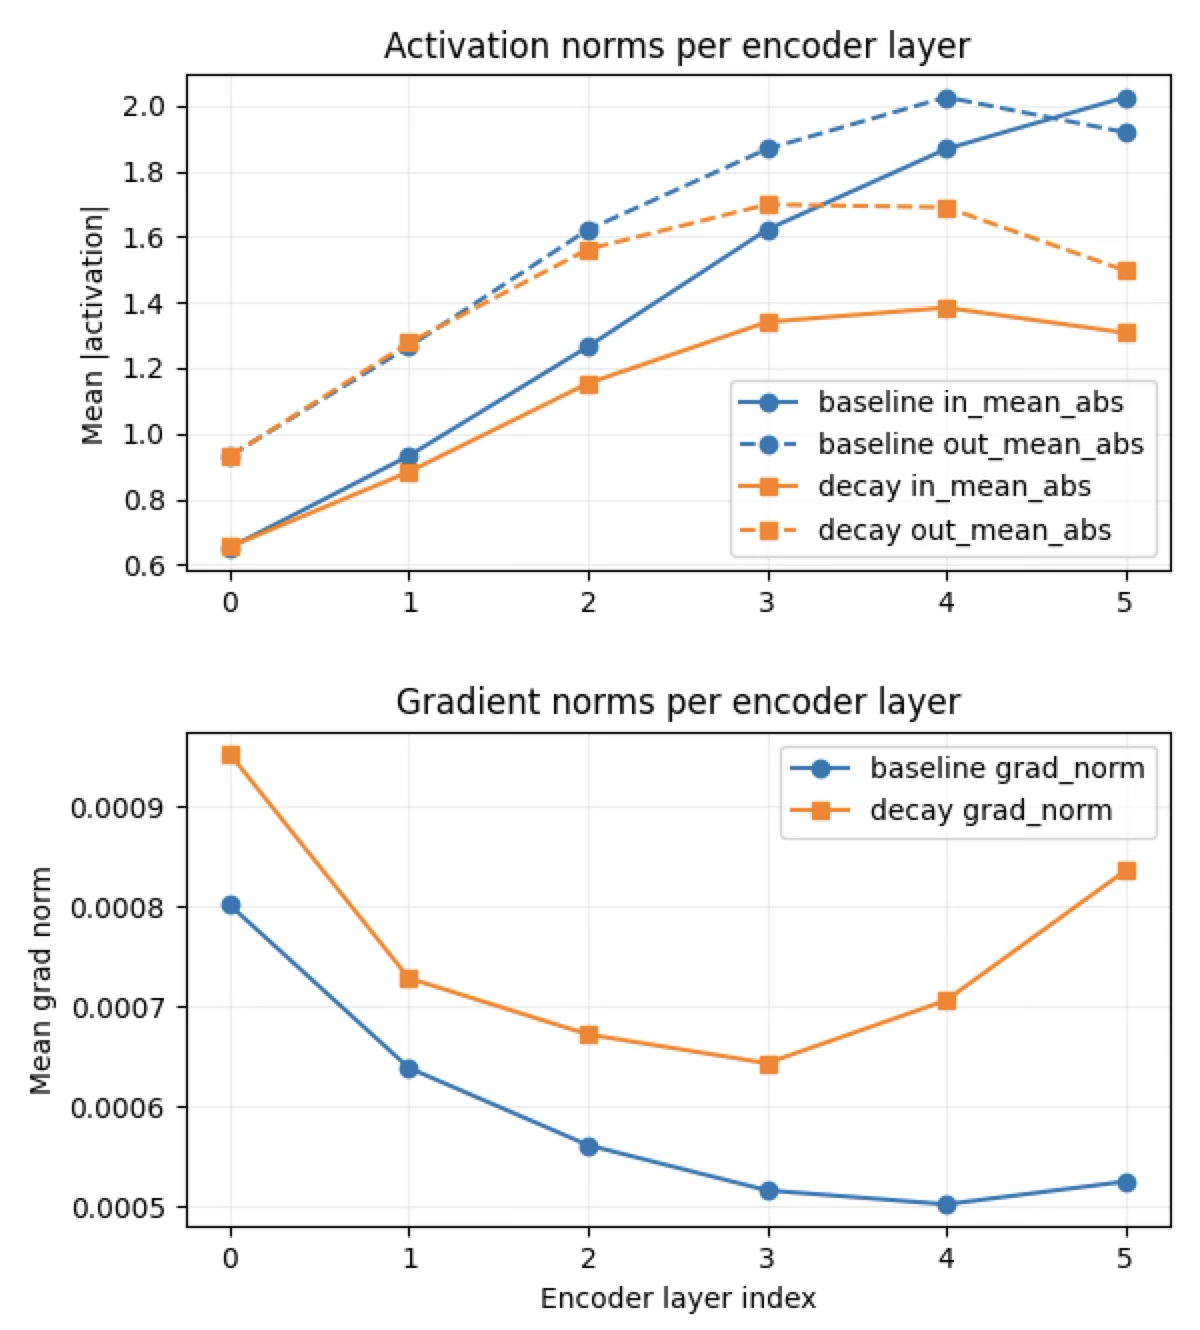
\includegraphics[height=0.85\textheight]{img/residual-norms.png}
\end{frame}

\begin{frame}{Backup --- Record 6, individual contributions \hfill \mut{\footnotesize median min}}
  \centering
  \begin{tabular}{@{}lr@{}}
    \toprule
    variant & median \\
    \midrule
    starting point (Record 5)     & $7.57$ \\
    RMSNorm only                  & $6.32$ \\
    Thinking rows only            & $4.22$ \\
    RMSNorm + Thinking rows       & $3.88$ \\
    \bottomrule
  \end{tabular}
\end{frame}

\begin{frame}{Backup --- thinking-row attention}
  \centering
  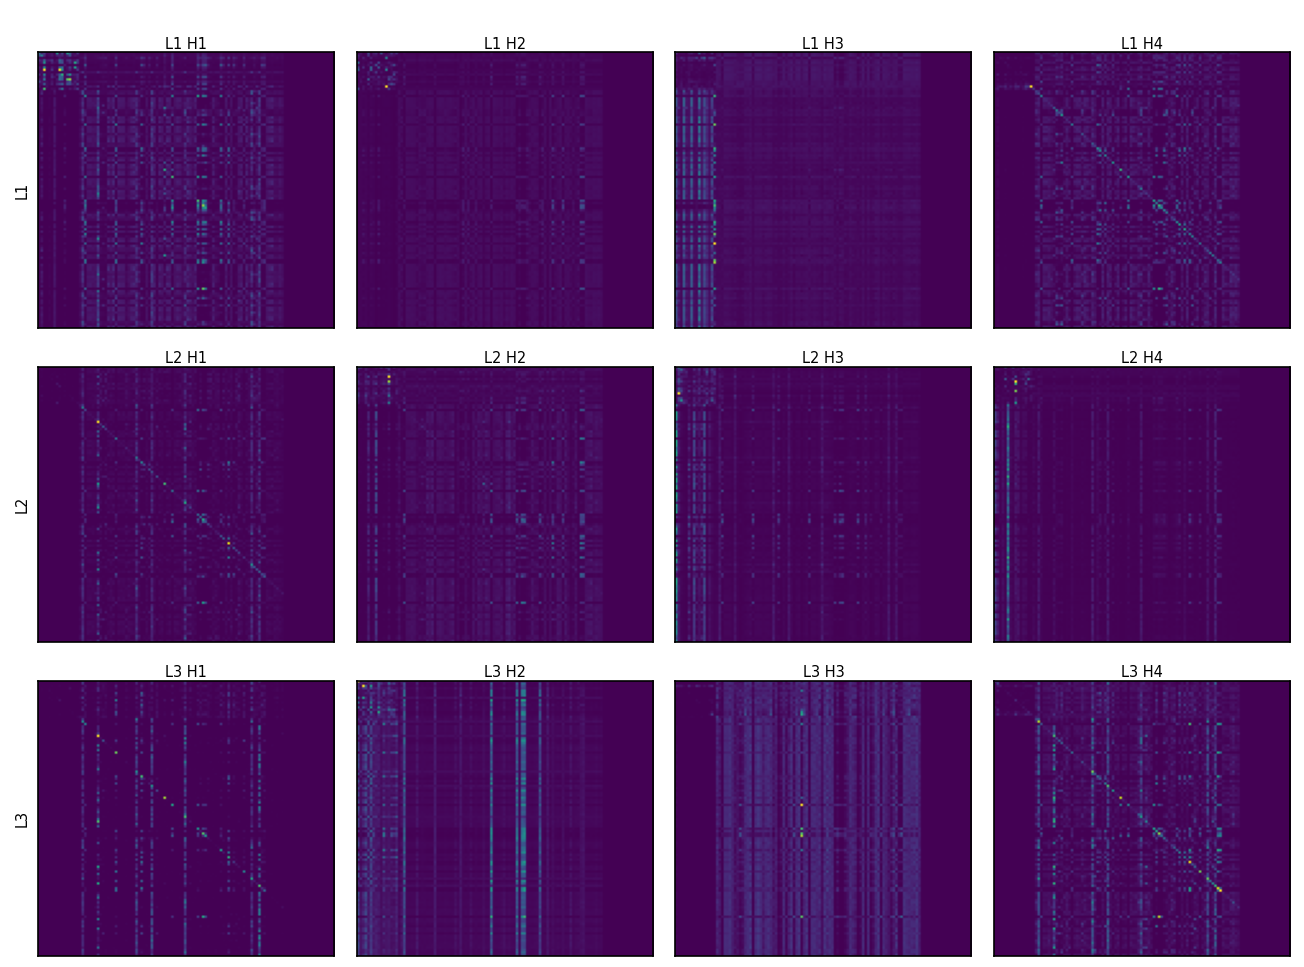
\includegraphics[height=0.85\textheight]{img/thinking-attention.png}
\end{frame}

\begin{frame}{Backup --- Record 9 autoresearch HPO}
  \centering
  \begin{tabular}{@{}lrr@{}}
    \toprule
    Hyperparameter & Before & After \\
    \midrule
    batch\_size         & $1$    & $2$    \\
    steps               & $64$   & $32$   \\
    l (encoder layers)  & $6$    & $5$    \\
    thinking\_rows      & $16$   & $24$   \\
    feature\_group\_size& $3$    & $5$    \\
    muon\_momentum      & $0.95$ & $0.96$ \\
    grad\_clip          & $1.0$  & $2.0$  \\
    \bottomrule
  \end{tabular}
\end{frame}

\begin{frame}{Backup --- full technique list}
  \tiny
  \begin{columns}[T]
    \begin{column}{0.5\textwidth}
      \begin{itemize}
        \item Muon optimizer
        \item Batched Muon zeropower for grouped QKV
        \item Explicit-QKV SDPA rewrite
        \item Pre-norm transformer blocks
        \item Compiled encoder-layer forward
        \item bf16 autocast (train + infer)
        \item TF32 matmul precision
        \item LR $10^{-4}\to10^{-3}$
        \item Embedding $192\to256$, heads $6\to4$
        \item Exponential residual decay
        \item Lower-precision RMSNorm
      \end{itemize}
    \end{column}
    \begin{column}{0.5\textwidth}
      \begin{itemize}
        \item 24 learnable thinking rows
        \item LAWA over 10 checkpoints
        \item sf-AdamW weight decay 0.01
        \item Repeated feature grouping (size 5)
        \item Autoresearch-driven HPO
        \begin{itemize}\tiny
          \item Layers $6\to5$
          \item Batch size $1\to2$, dump step $64\to32$
          \item Muon WD 0.1
          \item Muon momentum $0.95\to0.96$
          \item Gradient clip $1.0\to2.0$
          \item Mean feature pooling into decoder
        \end{itemize}
      \end{itemize}
    \end{column}
  \end{columns}
\end{frame}

\begin{frame}{Backup --- evaluation pipeline detail}
  \footnotesize
  \begin{itemize}
    \item \textbf{Subsampling:} $>100$ feats $\to$ 100 random; $>1000$ rows $\to$ 1000 stratified; fixed seed.
    \item \textbf{CV:} 5-fold \texttt{StratifiedKFold}, shuffled; labels integer-encoded per fold on train.
    \item \textbf{Preprocessing} (per fold, fit on train only):
      \begin{itemize}\footnotesize
        \item drop columns with $\le 1$ unique non-NaN value
        \item numeric: \texttt{to\_numeric} coercion + mean imputation
        \item categorical: ordinal encoding (unknown$\to$NaN) + most-frequent imputation
      \end{itemize}
    \item \textbf{Metric:} concat out-of-fold preds, \texttt{roc\_auc\_score} (binary / OvR), mean over 38 tasks.
    \item All randomness seeded with 11. Target $=0.8068462330697953$ (scikit-learn RandomForest through the same pipeline).
    \item \textbf{Verification:} new records are re-run on the same hardware at the same seed.
  \end{itemize}
\end{frame}

% ===========================================================================
\begin{frame}{Backup --- subsampling}
  \centering
  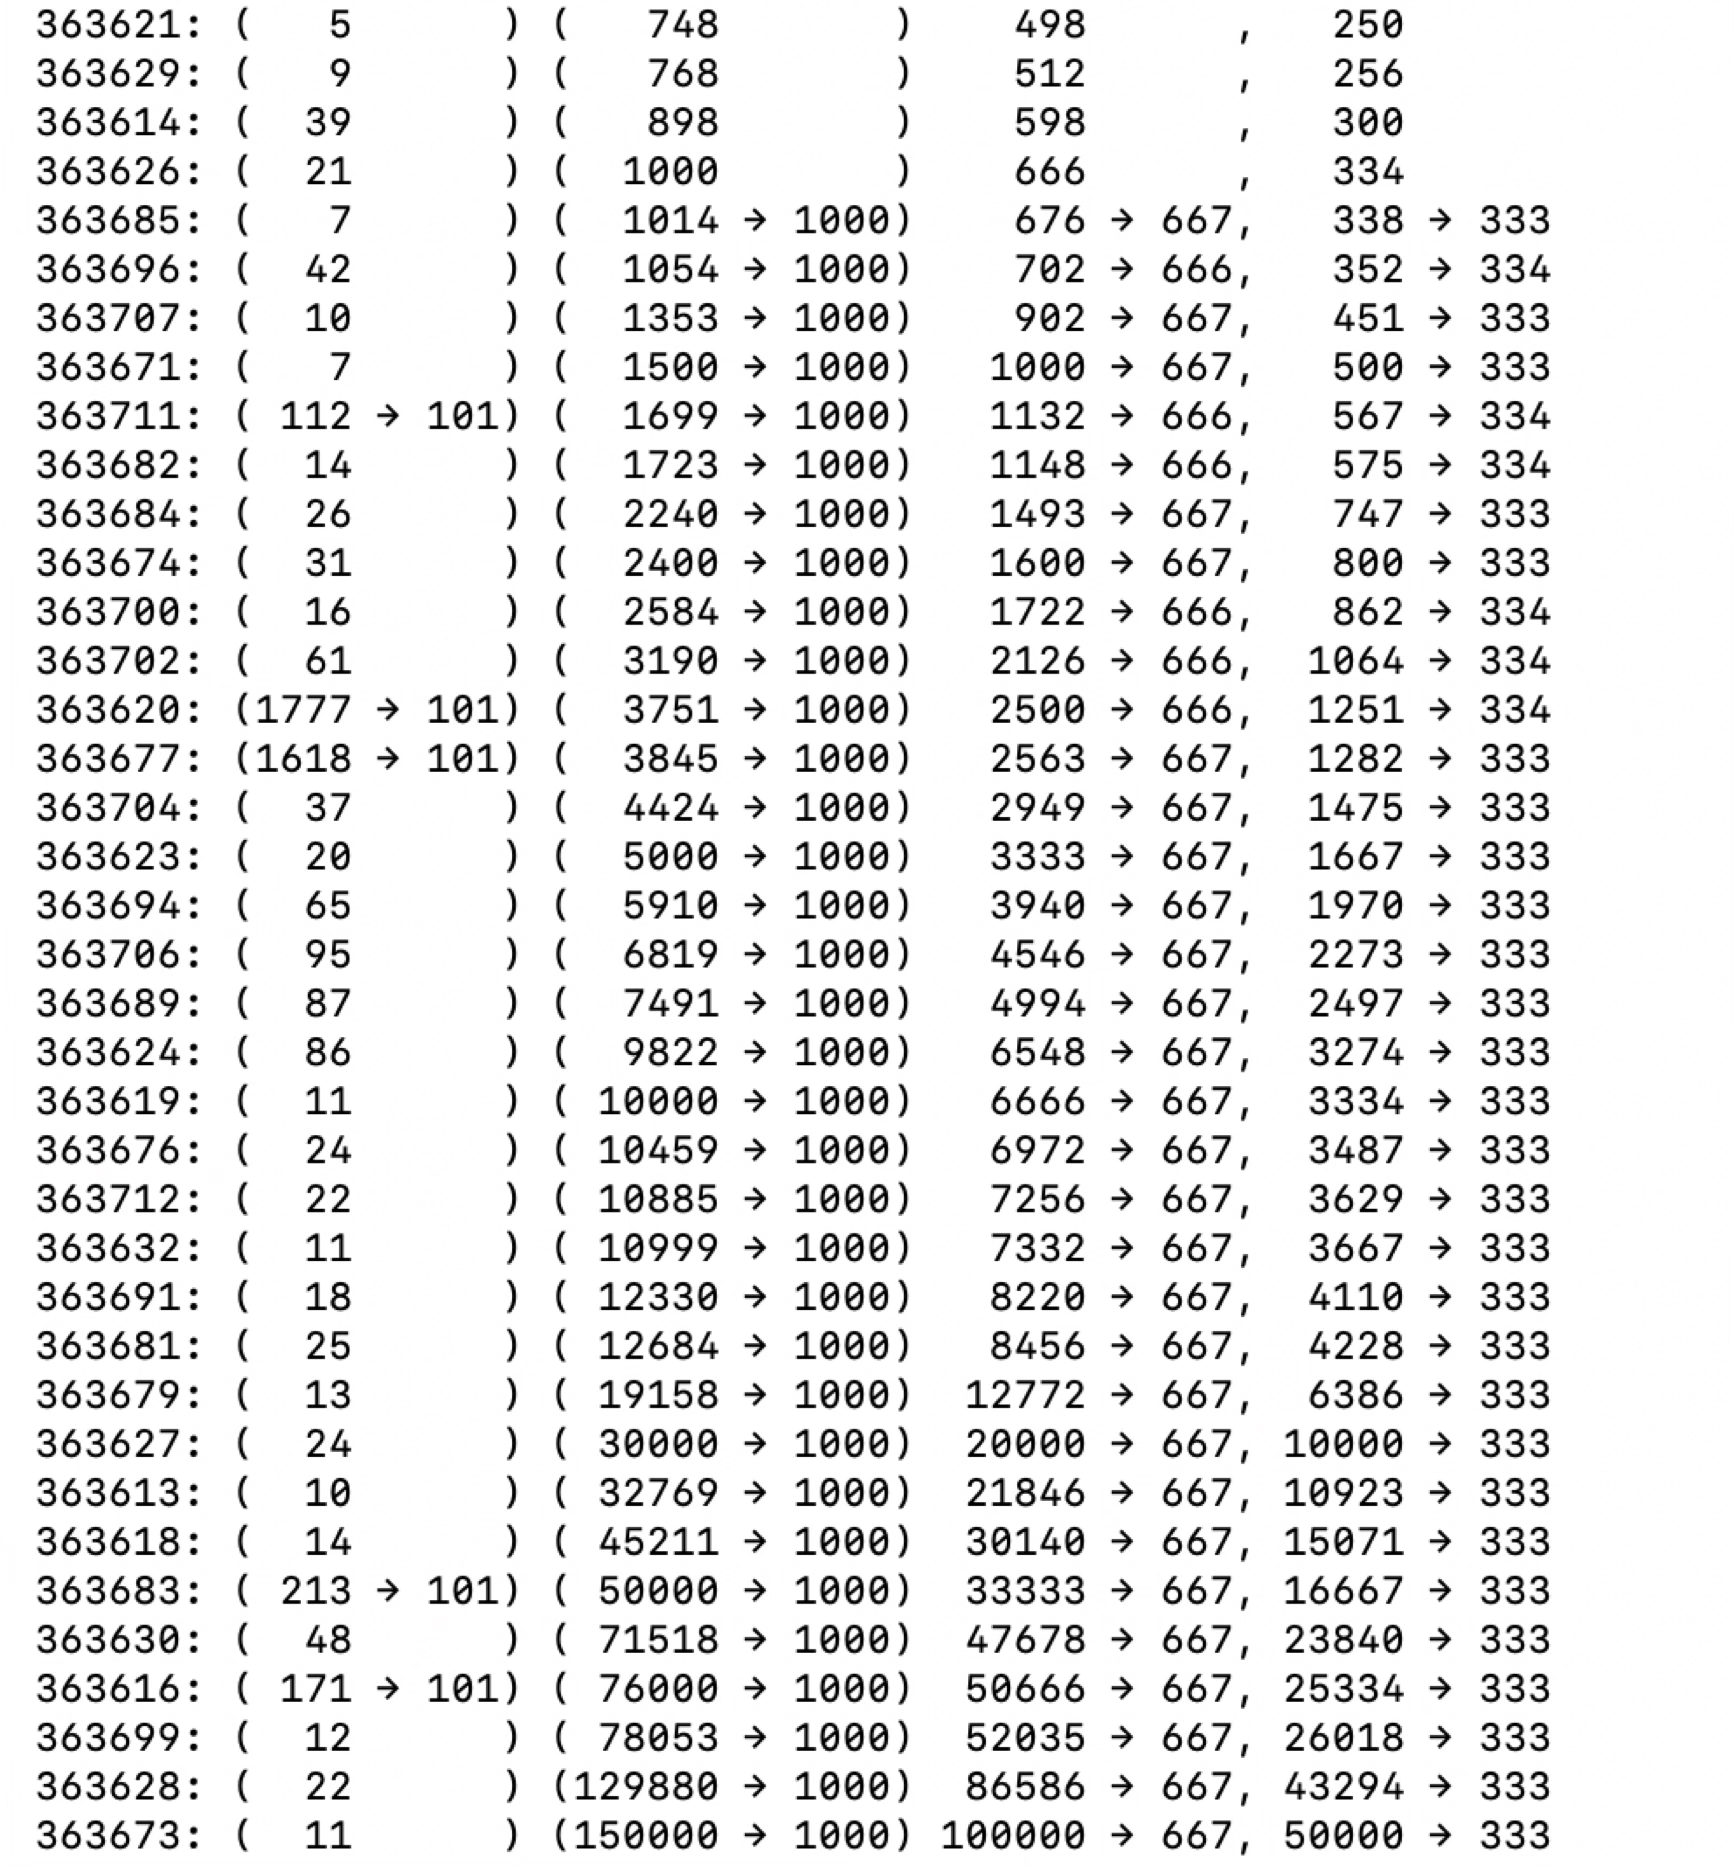
\includegraphics[height=7.2cm]{img/subsampled.png}
\end{frame}

% ===========================================================================
\begin{frame}{Backup --- the prior}
  \begin{itemize}
    \item Static dump of $256{,}000$ synthetic classification datasets
    \item Generated by the TabICL prior \cit{Qu '25}
    \item Each dataset: $1{,}000$ rows, $\le$20 features, $\le$8 classes
    \item Pre-generated; generation time excluded from the wallclock
    \item Held fixed across all records so far
  \end{itemize}
\end{frame}

% ===========================================================================
\begin{frame}{Backup --- differences from nanoTabPFN}
  \begin{itemize}
    \item Scaled-up evaluation limits: $5\times$ more datapoints, $10\times$ more features
    \item All 38 TabArena classification tasks via subsampling\\
      \mut{nanoTabPFN subsampled rows but filtered out feature-heavy datasets}
    \item nanoTabPFN: simple, educational code\\
      modded-nanoTabPFN: anything that speeds up training
  \end{itemize}
\end{frame}

% ===========================================================================
\begin{frame}{Backup --- what didn't work (reverted)}
  \begin{columns}[T]
    \begin{column}{0.5\textwidth}
      \begin{itemize}
        \item GoLU activation
        \item Xavier initialization
        \item Multi-GPU training
        \item Gradient checkpointing
        \item PISA/NSISA optimizer
      \end{itemize}
    \end{column}
    \begin{column}{0.5\textwidth}
      \begin{itemize}
        \item Softer softcap
        \item Self-compressing neural networks
        \item TabPFN v3 architecture
        \item Deterministic flagging
        \item Residual decay original param settings
      \end{itemize}
    \end{column}
  \end{columns}
\end{frame}

\end{document}
